\chapter{Adquisición Fonética en Dinámica Cortical}

\label{ch:phonetics}

\section{Introducción}


Se sabe que los humanos tienen la capacidad de discriminar fonemas y otras unidades lingüísticas clasificándolas sin importar la variabilidad evidenciada por diferentes hablantes con distintos tonos de voz y prosodia. Es más, dichas capacidades de clasificación se trasladan a ambientes ruidosos y reverberantes.

Aunque dicha competencia  podría ser atribuida en parte a la información proveniente de activaciones corticales originadas en fenómenos cognitivos de orden superior \cite{PMID:17451657}, por ejemplo, fenómenos de dimensión gramatical y semántica  \cite{OBLESER2011713,10.1093/cercor/bhp128} presentes en el lenguaje humano--más allá de las características fonéticas de la señal del habla--se  ha demostrado que una gran variedad de animales entrenados también tienen la capacidad de discriminar pares de fonemas categóricamente y de generalizar frente a situaciones novedosas~\cite{kuhl_1975, kuhl_1983, kluender_1998, pons_2006, hienz_1996, dent_1997, lotto_1997}. Por ejemplo, activaciones corticales en hurones revelan la existencia de una especialización espectro-temporal en \gls{a1} que tiene la capacidad de sostener la discriminación de varios fonemas del Inglés Americano \cite{mesgarani_2008}, aún cuando el estímulo fue distorsionado por ruido aditivo y reverberación \cite{mesgarani_2014A}.

Aún más notable es como algunas tareas de adquisición temprana de lenguaje--de extremada complejidad--como la segmentación de palabras desde el flujo del habla pueden ser realizadas por infantes de 8 meses de edad basándose simplemente en las relaciones estadísticas entre sonidos adyacentes en el habla \cite{Saffran1996StatisticalLB}. Después de sólo dos minutos de exposición a un flujo de habla continuo generado por un sintetizador de habla, los infantes mostraron adquisición y discriminación exitosa. Es más, en la fase de entrenamiento no se presentó información alguna acerca de los límites de las palabras que fuera más allá de de la estructura estadística de las reglas fonotácticas inmersas en el estímulo. Los infantes tampoco recibieron ningún tipo de supervisión externa o refuerzo que pudiera haber guiado o impulsado la tarea de adquisición fonética, la cual fue completamente incidental.

Dicha invarianza adquirida incidentalmente en la percepción fonética de los mamíferos se debe basar necesariamente en características neurofisiológicas y anatómicas de la corteza de los mamíferos. Las características que estimamos potencialmente relevantes son agrupadas en el presente trabajo a los fines de plantear nuestras hipótesis computacionales.




%% NOTE from GKT: I have removed the headings for each paragraph. It doesn't really help with the reading. Instead we
%% now have key phrases with emphasis (emph).

%% Also a bit of a word about LaTeX, I have found many paragraphs are not formatted nicely to take advantage of the editor
%% wrapping. This makes it very hard to change the text. You will notice through all sections that I have edited thus far
%% that each paragraph is now on a soft-wrapped line. There is no newline until the end of the paragraph. I will only use
%% hard newlines on comments such as this.



%It is well known that human beings can reliably discriminate phonemes as well as other linguistic units by categorizing them, despite considerable variability across different speakers with different pitches and prosody. Furthermore, this ability extends to noisy and reverberant environments.

%\reviewerfive{Although such proficiency could in part be attributed to top-down information \cite{PMID:17451657} originated in the grammatical and semantic \cite{OBLESER2011713,10.1093/cercor/bhp128} dimensions present in human language--beyond the phonetic features in the speech signal}--trained animals are also able to discriminate phoneme pairs categorically and to generalize in novel situations~\cite{kuhl_1975, kuhl_1983, kluender_1998, pons_2006, hienz_1996, dent_1997, lotto_1997}. For instance, \reviewertwo{cortical activations in naive ferrets revealed the existence} of spectro-temporal tuning in \gls{a1} with the capacity of supporting discrimination of many American English phonemes \cite{mesgarani_2008}, even when stimuli were distorted by additive noise and reverberation \cite{mesgarani_2014A}.

%%I added this paragraph to the intro
%\reviewerfour{It is even more remarkable that an extremely complex task of early language acquisition as is the segmentation of words from fluent speech, is fulfilled by 8-month-old infants based simply on the statistical relationships between neighboring speech sounds \cite{Saffran1996StatisticalLB}. With only 2 minutes of exposure to a continuous speech stream generated by a speech synthesizer, infants showed succesful phonetic acquisition and discrimination. Furthermore, in the training phase there was no acoustic information about word boundaries beyond the statistical structure in the phonotactic rules immerse in the stimuli, and the subjects received no external associative supervision or reinforcement which could have guided or boosted the phonetic acquisition task, which was entirely incidental}.

%% I hold this paragraph just in case we need it
%%How can cortical tissue show such physiological properties in response to complex auditory streams? This \reviewerfour{incidentally acquired} invariance in phonetic perception found in mammals must be grounded necessarily in anatomical and neurophysiological characterisitcs of the mammalian cortex. The features we foresee as potentially relevant will be described in the following section.

%\reviewerfour{This incidentally acquired invariance in phonetic perception found in mammals must be grounded necessarily in anatomical and neurophysiological characterisitcs of the mammalian cortex. The features we foresee as potentially relevant are brought together in order to pose our computational hypotheses}.




\section{Generación de Corpus}
\label{CorpGen}

Generamos corpus de 500 palabras utilizando diez vocabularios diferentes con palabras monosilabicas, bisilabicas y trisilábicas elegidas de manera aleatoria del idioma Inglés y utilizando el sintetizador \gls{festival} \cite{festival2014}.


Generamos archivos de marcado de lenguaje con SABLE \cite{sable}. Con tales archivos instruimos \gls{festival} para que genere corpus con 500  palabras de vacabularios de 5 palabras utilizando diez voces diferentes disponibles en el sintetizador.

La organización de los corpus presenta ciertas reglas y restricciones a los fines de evitar sesgoz en los procesos de entrenamiento. Las voces se van eligiendo secuencialmente (seudo-aleatoriamente) con la restricción de que ninguna voz se puede utilizar por segunda vez hasta que la totalidad de las voces hayan tenido su turno. Cada voz se utiliza para producir dos palabras por turno--de manera pseudo-aleatoria--y ninguna palabra es repetida hasta que todas las palabras son producidas por tal voz.


Utilizamos dos conjuntos de voces, cada uno con 10 voces de origen Inglés provistos por Festival. El primer conjunto consistia de 8 voces masculinas y 2 femeninas: \texttt{cmu\_us\_fem\_cg, cmu\_us\_gka\_cg, cmu\_us\_ksp\_cg, cmu\_us\_rxr\_cg, cmu\_us\_jmk\_cg, cmu\_us\_rms\_cg, cmu\_us\_slt\_cg, cmu\_us\_jmk\_arctic\_clunits, cmu\_us\_rms\_arctic\_clunits, cmu\_us\_slt\_arctic\_clunits}. El otro conjunto consistía de 5 voces masculinas y 5 femeninas: \texttt{cmu\_us\_ahw\_cg, cmu\_us\_aup\_cg, cmu\_us\_axb\_cg, cmu\_us\_eey\_cg, cmu\_us\_awb\_cg, cmu\_us\_bdl\_cg, cmu\_us\_clb\_cg, cmu\_us\_ljm\_cg, cmu\_us\_bdl\_arctic\_clunits, cmu\_us\_clb\_arctic\_clunits}.

Cada palabra en el archivo de audio es seguida por una brecha de silencio cuya duración equivale a la pronunciación de la palabra \texttt{cat} producida por la misma voz utilizada para producir la última palabra. Utilizamos el programa \texttt{text2wave} provisto por Festival para generar un archivo de extensión \texttt{wav} desde el archivo SABLE.

Generamos todos los datasets (archivos de audio de los corpus) utilizados en el presente trabajo para entrenar el \gls{el} y los \glspl{svm} y para probar el \gls{cstm} completo. Tal carpeta icluye un conjunto de 840 corpus distribuidos en dos corpus por cada configuración organizada por dos conjuntos de voces sintetizadas, tres condiciones silábicas y diez vocabularios distribuidos en 6 variantes acústicas aparte de los corpus en sus versiones originales. Las 6 variantes acústicas corresponden a: dos niveles de ruido blanco (19.8 dB y 13.8 dB \gls{snr} promedio \gls{rms} tasa de potensia), dos niveles de reverberación (\gls{rt} con valores de 0.61 segundos y 1.78 segundos) y variaciones de tono en ambas direcciones (de E a G y de E a C) \cite{dematties_dario_2019_2576130}.







%We generate corpora of 500 words with mono, di and trisyllabic randomly chosen English words from \reviewerfour{10 different vocabularies of five words
%for each syllabic condition} using \gls{festival} Synthesis \cite{festival2014}.

%%\begin{itemize}
	%%\item Monosyllabic vocabulary: \textit{map, dog, mouse, with, truck.} % and \textit{truck}.
	%%\item Disyllabic vocabulary: \textit{answer, doctor, teacher, summer, tennis.}  %and \textit{tennis}.
	%%\item Trisyllabic vocabulary: \textit{computer, telephone, rectangle, tomato, magazine.} % and \textit{magazine}.
%%\end{itemize}

%%\todo[inline]{Silvio: can not see how these 15 words generate 500 words. Either I am missing something obvious or we need additional explanations}

%We generate \reviewertwo{cross synthesizer mark-up-language files} with SABLE \cite{sable}.
%In such files, we instruct \gls{festival} to generate corpora with 500 words from vocabularies of
%5 words uttered by 10 different voices available from the synthesizer.

%The organization of the corpora has certain rules and restrictions in order to avoid biases in the training processes.
%The voices are sequentially chosen (pseudo-randomly) with the restriction that no voice could utter a second time until all the voices had uttered in their turns. Every voice utters two words per turn--in pseudo-random order--and no word is repeated until all the words are used by such voice. 

%\reviewerfour{We use two sets of 10 different English speaking voices, each provided by Festival. Set one consisted of 8 male and 2 female voices: \texttt{cmu\_us\_fem\_cg, cmu\_us\_gka\_cg, cmu\_us\_ksp\_cg, cmu\_us\_rxr\_cg, cmu\_us\_jmk\_cg, cmu\_us\_rms\_cg, cmu\_us\_slt\_cg, cmu\_us\_jmk\_arctic\_clunits, cmu\_us\_rms\_arctic\_clunits, cmu\_us\_slt\_arctic\_clunits}. Set two had 5 male and 5 female voices: \texttt{cmu\_us\_ahw\_cg, cmu\_us\_aup\_cg, cmu\_us\_axb\_cg, cmu\_us\_eey\_cg, cmu\_us\_awb\_cg, cmu\_us\_bdl\_cg, cmu\_us\_clb\_cg, cmu\_us\_ljm\_cg, cmu\_us\_bdl\_arctic\_clunits, cmu\_us\_clb\_arctic\_clunits}}.

%Every word in the audio file is followed by a silence gap whose time is equivalent to the uttering time of the monosyllabic word \textit{cat}, uttered by the same voice used for the last word. We use the \texttt{text2wave} program provided by Festival in order to generate a \texttt{wav} file from the SABLE file.

%We generated all the datasets (audio file corpora) employed in the present research to train the \gls{el} and the \glspl{svm} and to test the complete \gls{cstm}. This folder includes a set of 840 corpora which are distributed in 2 corpora for each configuration organized by 2 sets of synthesized voices, 3 syllabic conditions and 10 vocabularies all distributed in 6 acoustic variants, beyond the original version of the corpora. The 6 acoustic variants corresponds to: two levels of white noise (19.8 dB and 13.8 dB \gls{snr} average \gls{rms} power rate), two levels of reverberation (\gls{rt} value of 0.61 seconds and 1.78 seconds) and variations of pitch on both directions (from E to G and from E to C) \cite{dematties_dario_2019_2576130}.





%%We generate a corpora of 500 words with mono, di and trisyllabic randomly chosen English words with vocabularies of five words
%%using \gls{festival} Synthesis \cite{festival2014}.

%%\begin{itemize}
	%%\item Monosyllabic vocabulary: \textit{map, dog, mouse, with, truck.} % and \textit{truck}.
	%%\item Disyllabic vocabulary: \textit{answer, doctor, teacher, summer, tennis.}  %and \textit{tennis}.
	%%\item Trisyllabic vocabulary: \textit{computer, telephone, rectangle, tomato, magazine.} % and \textit{magazine}.
%%\end{itemize}

%%%\todo[inline]{Silvio: can not see how these 15 words generate 500 words. Either I am missing something obvious or we need additional explanations}

%%We generate a \reviewertwo{cross synthesizer mark-up-language file} with SABLE \cite{sable}.
%%In this file, we instruct \gls{festival} to generate a corpus with 500 words from a vocabulary of
%%5 words uttered by 10 different voices (8 males and 2 females) available from the synthesizer.

%%The organization of the corpus has certain rules and restrictions in order to avoid biases in the training processes.
%%The voices are sequentially chosen (pseudo-randomly) with the restriction that no voice could utter a second time until all the voices had uttered in their turns. Every voice utters two words per turn--in pseudo-random order--and no word is not be repeated until all the words are used by such voice. 

%%We use the following English speaking voices provided by Festival: \texttt{cmu\_us\_fem\_cg, cmu\_us\_gka\_cg, cmu\_us\_ksp\_cg, cmu\_us\_rxr\_cg, cmu\_us\_jmk\_cg, cmu\_us\_rms\_cg, cmu\_us\_slt\_cg, cmu\_us\_jmk\_arctic\_clunits, cmu\_us\_rms\_arctic\_clunits, cmu\_us\_slt\_arctic\_clunits}.

%%Every word in the audio file is followed by a silence gap whose time is equivalent to the uttering time of the monosyllabic word \textit{cat}, uttered by the same voice used for the last word. We use the \texttt{text2wave} program provided by Festival in order to generate a \texttt{wav} file from the SABLE file.




\section{Análisis Multiresolución Espectro-Temporal de Sonidos (AMRETS)}
\label{mrstsa}

Implementamos la etapa inicial del \gls{mrstsa} con la aplicación de la \gls{fft} al vector de audio con una ventana de muestreo diferente para cada resolución. Luego extraemos la densidad espectral de potencia desde cada resolución. Aplicamos \gls{fft} a los archivos de audio con un período de muestreo de 8 milisegundos, para ello utilizamos el paquete FFTW \cite{FFTW05, fftw} con ventanas temporales de 8, 16, 32, 64 y 128 milisegundos. De esta manera obtenemos un análisis espectral de la señal de audio de resolución múltiple con alta resolución espectral y baja resolución temporal para ventanas grandes y vice versa. Tales diferencias en las ventanas temporales en la aplicación de la \gls{fft} incorporan--al mismo tiempo--filtros pasa-bajo de fuga con una constante de tiempo diferente para cada resolución representando la pérdida de fase en el nervio auditivo. Luego aplicamos \gls{mfb} con 128 elementos a cada espectro a los fines de representar el análisis espectral realizado por el banco de filtros cocleares (Fig.\ref{fig:MRSTSA}).

%We implemented the initial stage in the \gls{mrstsa} with the application of \gls{fft} to the audio vector with a different sample window for each resolution. We then extracted the power spectral density from each resolution. We applied \gls{fft} to the audio files with a sample period of 8 milliseconds, to that end we used the FFTW package \cite{FFTW05, fftw} with time windows of 8, 16, 32, 64 and 128 milliseconds. In this way we obtained a multiresolution spectral analysis of the audio signal, with high spectral and low temporal resolution for wider sample windows and vice versa. Such different time windows in the \gls{fft}, incorporated--at the same time--leakage low-pass filters with a time constant for each resolution accounting for decrease of phase-locking in the auditory nerve. We then applied a \gls{mfb} with 128 elements to each spectrum in order to represent the spectral analysis performed by the cochlear filter bank (Fig.\ref{fig:MRSTSA}).

\begin{figure}[h!]
    \centering
    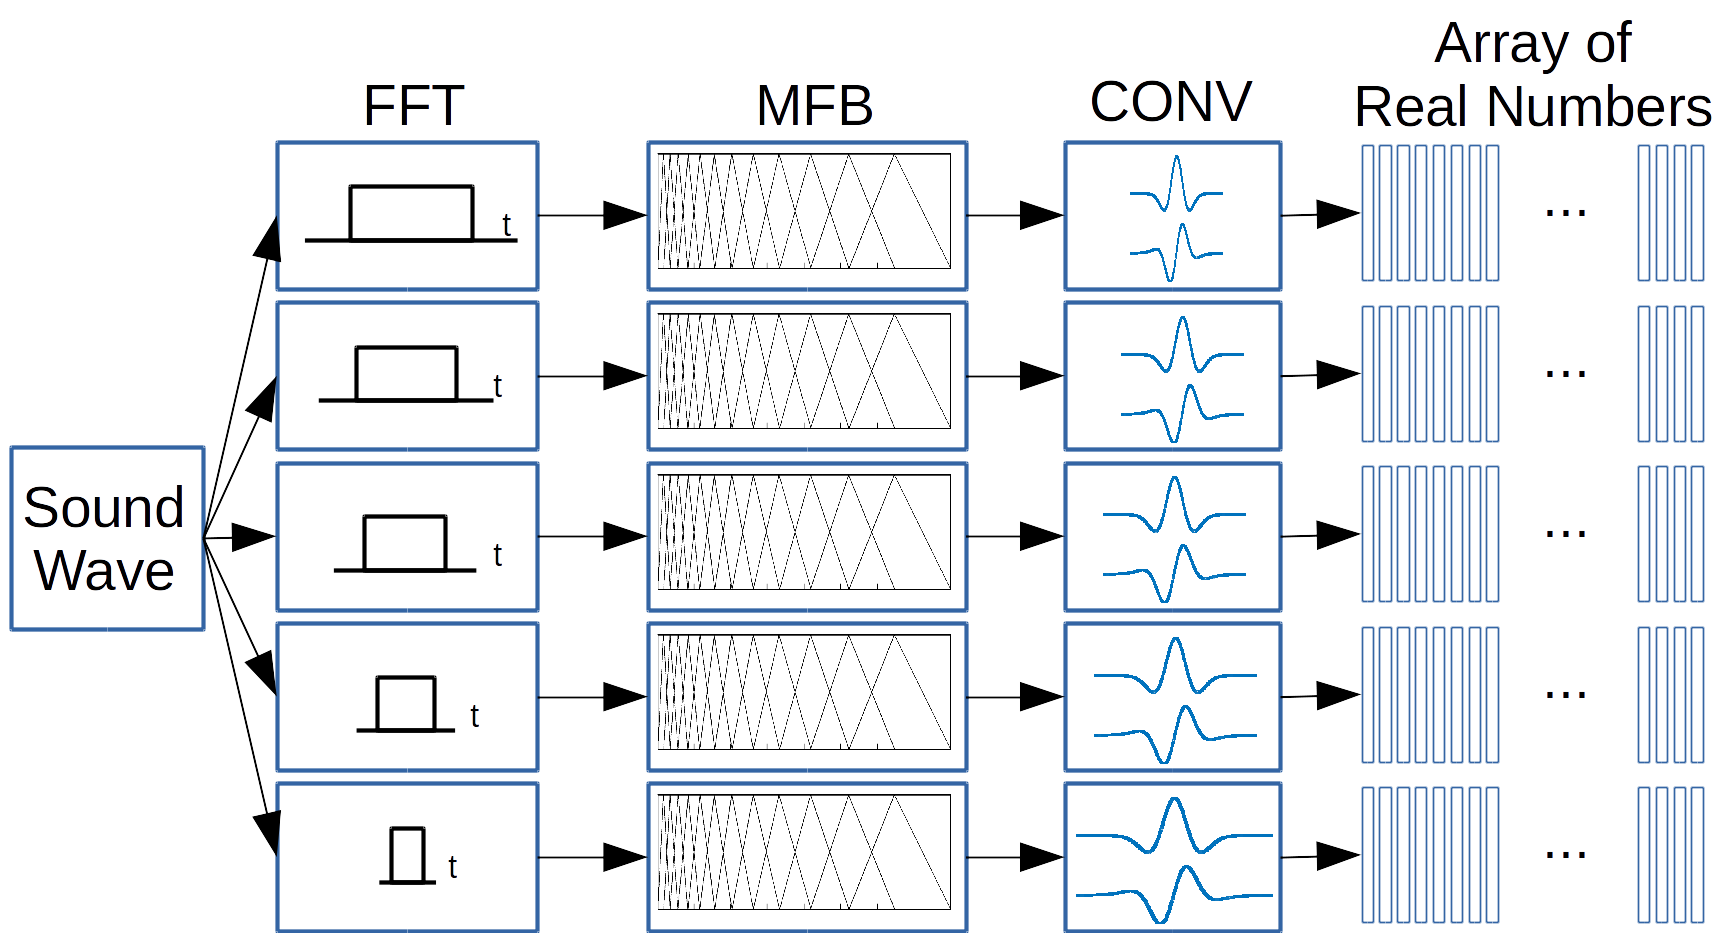
\includegraphics[width=0.8\textwidth]{MRSTSA.png}
    \caption{Algoritmo \glsfirst{mrstsa}. Las ondas de sonido son procesadas por \glspl{fft} con ventanas de tiempo diferentes, luego cada espectro es procesado por
    un \glsfirst{mfb} y cada resolución es convolucionada con una señal compleja con un coeficiente diferente. Luego, el coeficiente de cada filtro
    es obtenido computando el módulo desde la convolución y aplicando control automático de ganancia.}
    %\caption{\glsfirst{mrstsa} algorithm. Sound waves are processed by \glspl{fft} with different time windows, then each spectrum is processed by
    %a \glsfirst{mfb} and each resolution is convolved with a complex signal with a different coefficient. Then, each filter coefficient
    %is obtained computing the modulus from the convolution and then applying a authomatic gain control.}
    \label{fig:MRSTSA}
\end{figure}

Luego, convolucionamos cada resolución obtenida en el último paso a lo largo de su eje tonotópico con una función multiresolución compleja cuya parte real es un sobrero Mexicano simétrico y su parte imaginaria es su transformada antisimétrica de Hilbert. Los coeficientes de la función son 10 para la ventana de tiempo de 8 ms, 8 para la ventana de tiempo de 16 ms, 6 para la ventana de tiempo de 32 ms, 4 para la ventana de tiempo de 64 ms y 2 para la ventana de tiempo de 128 ms (Fig.\ref{fig:MRSTSA}). Con esta estrategia incorporamos el fenómeno de simetría \cite{shamma_1993}, ancho de banda \cite{schreiner_1990} y selectividad a la modulación de frecuencia \cite{shamma_1993,heil_1992,mendelson_1985} hallada en \gls{a1} e incorporado en el algoritmo original \cite{wang_1995}.

%Then, we convolved each resolution obtained in the last step along its tonotopic axis with a complex multiresolution function whose real part was a symmetric Mexican hat function and its imaginary part was its antisymmetric Hilbert transform. The function coefficients are 10 for the 8 ms time window, 8 for the 16 ms time window, 6 for the 32 ms time window, 4 for the 64 ms time window and 2 for the 128 ms time window (Fig.\ref{fig:MRSTSA}). With this strategy we incorporated the phenomena of symmetry \cite{shamma_1993}, bandwidth \cite{schreiner_1990} and frequency modulation selectivity \cite{shamma_1993,heil_1992,mendelson_1985} found in \gls{a1} and incorporated in the original algorithms \cite{wang_1995}.

Obtuvimos la magnitud de cada convolución y aplicamos normalización a cada ventana de tiempo como un control automático de ganancia para priorizar la información entregada por la configuración espectral y no por los valores absolutos entregados por los filtros. Por medio de este mecanismo estamos teniendo en cuenta las propiedades químicas y mecánicas de las células poliosas en el oído interno de los mamíferos las cuales constituyen un mecanismo de transducción el cual parece adaptarse a la historia reciente en los estímulos de manera que puede afectar su ganancia \cite{eatock_2000,holt_2000,le_goff_2005}. Decidimos ser conservativos y no incluir la dimensión de intensidad de sonido sólo incluyendo la silueta en las respuestas de los filtros. 

%We obtained the magnitude of each convolution and applied normalization to each time window as a mean of automatic gain control in order to prioritize the information delivered by the spectral configuration and not the absolute values delivered by the filters. By means of this constraint we account for the mechanical and chemical properties of hair cells in the mammalian inner ear which constitute a transduction mechanism that appears to adapt to recent stimulus history in a way that can affect its gain \cite{eatock_2000,holt_2000,le_goff_2005}. We decided to be conservative, not including sound intensity dimension but just the shape of the filter responses.

Por medio de este procedimiento desde el archivo de audio obtuvimos una respuesta multiresolución espectro-temporal compuesta por un arreglo de 128 columnas--una columna por filtro--y 5 filas--una fila por resolución--con números reales cuyo rango se encuentra entre 0 y 1, para cada paso de tiempo.

%By this procedure we obtained from the audio file a multiresolution spectro-temporal response composed by an array of 128 columns--one column per filter--and 5 rows--one row per resolution--with real numbers which range from 0 to 1, for each time step.




\section{Implementación}

\subsection{Análisis Multiresolución Espectro-Temporal de Sonidos (AMRETS)}

Aplicamos la \gls{fft} a los archivos de audio con un período de muestreo de 8 milisegundos.
A tales efectos utilizamos le paquete FFTW \cite{FFTW05, fftw} con ventanas de tiempo de 8, 16, 32, 64 y 128 milisegundos a los fines de obtener un análisis espectral de potensia de miltiple resolución de la señal.
Adicionalmente, aplicamos la técnica de Banco de Filtros Mel con 128 filtros para cada resolución espectral y convolucionamos tales filtros a lo largo de su ejes tonotópicos. Para la convolución utilizamos una función compleja de resolución múltiple cuya parte real is una función de Sombrero Mexicano y su parte imaginaria es su transformación de Hilbert.

Los valores de los coeficientes de la función son 10 para un tiempo de ventana de 8 milisegundos, 8 para un tiempo de ventana de 16 ms, 6 para un tiempo de ventana de 32 milisegundos, 4 para un tiempo de ventana de 64 milisegundos y 2 para un tiempo de ventana de 128 milisegundos.
Luego computamos la magnitud de la convolución y normalizamos en cada paso temporal.
Por medio de este procedimiento obtenemos desde el archivo de audio una respuesta espectro-temporal de multiple resolución compuesta por un arreglo de 128 columnas--una columna por filtro--y 5 filas--una fila por resolución--de npumeros reales con un rango de 0 a 1 fara cada paso temporal.


%We apply \gls{fft} to the audio files with a sample period of 8 milliseconds.
%We use the FFTW package \cite{FFTW05, fftw}
%with time windows of 8, 16, 32, 64 and 128 milliseconds in order to obtain
%a multiresolution power spectral analysis of the signal.
%%We then applied 
%In addition, we apply the Mel Filter-Bank technique with 128 filters to each
%spectral resolution and convolve such filters along their tonotopic axis.
%For the convolution, we use a multiresolution complex function whose real part
%is a Mexican hat function and its imaginary part is the corresponding Mexican hat Hilbert transformation.
%%-Fig. \ref{fig:Multi}.

%%\begin{figure}[h!]
    %%\centering
    %%\includegraphics[width=0.7\textwidth]{Multi.png}
    %%\caption{Multiresolution complex kernels. Such kernels are convolved with Mel Filter Bank outputs along their tonotopic axis.
	    %%Each kernel has a different coefficient
    %%and is convolved with its corresponding power spectral resolution.
    %%The function coefficients are 10 for 8 ms time window, 8 for 16 ms time window, 6 for 32 ms time window, 4 for 64 ms time window
    %%and 2 for 128 ms time window.}
    %%\label{fig:Multi}
%%\end{figure}

%The function coefficients are 10 for the 8 ms time window, 8 for the 16 ms time window, 6 for the 32 ms time window, 4 for the 64 ms time window
%and 2 for the 128 ms time window. We then compute the magnitude from the convolution and normalize in each time step.
%By means of this procedure we obtain from the audio file a multiresolution spectro-temporal response composed by
%an array of 128 columns--one column per filter--and 5 rows--one row per resolution--with real numbers which range from
%0 to 1, for each time step.



\subsection{Encoder Layer (EL)}

Implementamos un \gls{el} con 225 \glspl{csom} organizados en un arraglo de dos dimensiones de 15 por 15 \glspl{cc}.
Cada \gls{cc} es automáticamente distribuida utilizando ubicaciones individuales a lo largo de sus entradas aferentes de manera uniforme.
Cada \gls{cc} recibe información aferente a través de campos receptivos aferentes bi-dimensionales de 5 por 227 filtros centrados en posiciones individuales sobre el \gls{mrstsa}.
Abilitamos la propiedad de envoltura (wraparound) para lograr que cada campo receptivo ocupe el arreglo del \gls{mrstsa} por completo.
También instruimos a cada columna para que reciba solo 31 entradas, lo cual constituye un porcentaje menor del campo receptivo.
Las entradas aferentes individuales para cada \gls{cc} son escojidas aleatoriamente durante el proceso de inicialización del \gls{el}.

Para esta instancia del modelo, implementamos solo ramificaciones dendríticas laterales ya que no existe más \glspl{cl} de donde traer información por medio de ramificaciones dendríticas apicales.
Configuramos cada \gls{cc} para que tenga un campo receptivo lateral de 9 por 9 \glspl{cc} vecinas y para recibir información de 72 de las 81 \glspl{cc} in el campo receptivo--un 90\% del campo receptivo.


Cada \gls{cc} está compuesta de un arreglo bi-dimensional con 15 por 15 (225) unidades neuronales y cada unidad en una columna podría ser conectada potencialmente con solo 6 unidades neuronales en cada columna vecina vinculada.
De esta manera, cada unidad neuronal en una \gls{cc} termina teniendo 72 ramificaciones dendríticas con 6 conecciones potenciales cada una (432 sinapsis potenciales distantes por unidad celular).
Tales conecciones potenciales se seleccionan de manera aleatoria para cada unidad celulary para cada rama dendrítica en la célula durante el proceso de inicialización del Encoder. El \gls{el} consiste de 50625 unidades celulares con 1569375 sinapsis potenciales y 21870000 sinapsis distantes.
Tales especificaciones determinan el npumero de parámetros libres del modelo, sin embargo, es importante resaltar que las sinapsis distantes representan conecxiones potenciales desde las que solo un pequeño porcentaje tiene un peso sináptico significativo como para ser consideradas conexiones establecidas.
Las sinapsis débiles son periódicamente descartadas por medio de procesos homeostáticos in la red dejando las dendritas distantes con una conectividad dispersa en los campos receptivos. Dispersiones típicas in tales conectividades podrían exeder el 90\%.

Entrenamos el \gls{el} utilizando corpus de 500 palabras generados por el procedimiento descripto en la sección \nameref{CorpGen}.
El procedimiento de entrenamiento consiste de 4 stapas y para cada etapa el \gls{el} recibe el mismo corpus 4 veces.

Durante cada etapa de aprendizaje, ciertos parámetros--como las tasas de aprendizaje en sinapsis próximas y distantes y la iteracción intracolumnar lateral--son decrementadas progresivamente exponencialmente desde un valor inicial, el cual también es decrementado en cada etapa sucesiva.
Una etapa adicional es ejecutada con los parámetros de aprendizaje fijos.

La dispersión en la activación para cada \gls{cc} es 99\% (solo 2 unidades neuronales de las 225 podrían ser activadas por medio de eventos normales de activación).
Por otro lado, la exitación aferente afecta el 10\% de las unidades dentro de los cúmulos en cada \gls{cc}
(22 unidades neuronales, las cuales podrían ser activadas en caso de un \gls{mfe}; Fig. \ref{fig:Activation}).

Cada \gls{cc} esta compuesta de un arreglo bi-dimensional con 15 por 15 (225) unidades neuronales y
cada unidad en una columna podría ser connectada potencialmente con sólo 6 unidades neuronales desde cada columna vecina vinculada.
(432 sinapsis distales por unidad celular).


%We implement an \gls{el} with 225 \glspl{csom} arranged in a two-dimensional
%array of 15 by 15 \glspl{cc}. Each \gls{cc} is automatically distributed using individual locations along its afferent inputs in a uniform way.
%Each \gls{cc} receives afferent information by means of
%two-dimensional afferent receptive fields of 5 by 227 filters centered at individual locations over the \gls{mrstsa}.
%We enable the wraparound property in order to make each receptive field span the entire
%\gls{mrstsa} array.
%We also instruct each column to receive only 31 inputs, which is a minor percentage of such
%receptive field.
%Individual afferent inputs for each \gls{cc} are chosen randomly in the \gls{el} initialization. 

%For this model instance we implement only distal lateral dendritic branches since there are
%no more \glspl{cl} from which to bring information through apical dendritic branches.
%We configure each \gls{cc} to have a lateral receptive field with 9 by 9 neighboring \glspl{cc}
%and to receive information from 72 of the 81 \glspl{cc} in the receptive field--a 90\% of the receptive field.

%Each \gls{cc} is composed of a two-dimensional array with 15 by 15 (225) neural units and
%each unit in a column could be potentially connected with only 6 neural units from each linked neighboring column. 
%That is, each neural unit in a \gls{cc} ends up with 72 lateral dendritic branches with 6 potential connections each
%(432 distal potential synapses per cellular unit).
%Such potential synapses are randomly chosen for each neural cell and for each dendritic branch in the cell during the Encoder initialization procedure.
%The \gls{el} consists of 50625 cellular units with 1569375 proximal synapses and 21870000 distal synapses.
%\reviewerfour{Such specifications state the number of free parameters of the model, but it is important to highlight that distal synapses represent
%potential connections from which only a small percentage has a significant synaptic weight as to be considered as an established connection.
%Weak synapses are periodically pruned by means of homeostatic processes in the network leaving distal dendrites with a sparse connectivity in the receptive fields.
%Typical sparseness in such connectivity matrices could exceed the 90\%.}

%We train the \gls{el} using a 500 word corpora generated by the procedure described in section \nameref{CorpGen}.
%The training procedure consists of 4 stages and for each stage the \gls{el} receives the same corpus 4 times.

%During each learning stage, certain parameters--such as the learning rates in proximal and distal synapses and the lateral
%intra-column interaction--are exponentially and progressively decreased from an initial value, which also decreases
%for each successive stage.
%An additional stage is executed with the learning parameters fixed.

%The sparsity in the activation for each \gls{cc} is 99\% (just 2 neural units out of 225 could be active for normal activation events).
%On the other hand, the afferent excitation affects 10\% of the units inside the clusters in each \gls{cc}
%(22 neural units, which could be activated in case of a \gls{mfe}; Fig. \ref{fig:Activation}).








\subsection{Clasificación por medio de Support Vector Machine (SVM)}

Utilizamos supervisión con clasificación por medio del método \gls{svm}, recibiendo las salidas de cada algoritmo \cite{CC01a, libsvm}. Hacemos eso para probar las propiedades de invarianza en las características fonéticas abstraidas por el \gls{el} en comparación con las propiedades fonéticas abstraidas por el \gls{mrstsa}, 
(Fig. \ref{fig:Experiment}).

Utilizamos las brechas temporales de silencio entre palabras consecutivas en las salidas del \gls{mrstsa} para introducir marcas y así detectar el pricipio y el final de cada palabra.

Luego, producimos un vector por palabra en el corpus sumando la actividad en el \gls{mrstsa} así como en el \gls{el} entre marcas consecutivas
y utilizamos tales vectoresjpara entrenar ambos clasificadores (el que recibe las salidas provenientes desde el \gls{mrstsa} y el que las recibe desde el \gls{el}).

Luego, escalamos los vectores--como la documentación del \gls{libsvm} sugiere--para mejorar el desempeño en la clasificación.
Entrenamos y probamos los clasificadores \gls{svm} utilizando validación cruzada sobre 5 secciones y los configuramos para utilizar un kernel linear con un parámetro $C$ el cual barremos para encontrar el mejor modelo entrenado para cada clasificador.



%We use supervision by means of the \gls{svm} classification
%method, receiving the outputs from each algorithm \cite{CC01a, libsvm}. We do this to test the invariance properties in the phonetic features abstracted by the \gls{el} in comparison
%with the phonetic features abstracted by the \gls{mrstsa}, 
%(Fig. \ref{fig:Experiment}).

%We use the silent temporal gaps between consecutive words in the \gls{mrstsa} outputs in order to introduce marks to
%detect the beginning and end of each word.

%We then produce a vector per word in the corpus summing the activity in the \gls{mrstsa} as well as in the \gls{el} between consecutive marks
%and use such vectors to train both classifiers (the one receiving outputs from the \gls{mrstsa} and the one receiving outputs from the \gls{el}).

%Afterwards, we scale the vectors--as the \gls{libsvm} documentation suggests--
%so as to improve the classification performance.
%We train and test the \gls{svm} classifiers using 5-fold cross-validation
%and configure them to use a linear kernel with one parameter $C$ which
%we swept to find the best trained model for each classifier.


\section{Experimentos}

En el trabajo presentado en este capítulo, estudiamos el nivel de invarianza en las características fonéticas abstraidas por el \gls{el} a través de la comparación de tales representaciones con las características auditivas espectro-temporales devueltas por el algoritmo \gls{mrstsa}. A tal fin, evaluamos los rasgoz devueltos por cada algoritmo frente a diferentes tareas de clasificación de palbras. A los fines de probar el desempeño de clasificación en cada algoritmo, utilizamos la técnica \gls{svm}--sección \nameref{model-implementation}--con el perfil experimental descripto en la Fig. \ref{fig:Experiment}.

\begin{figure}[h!]
    \centering
    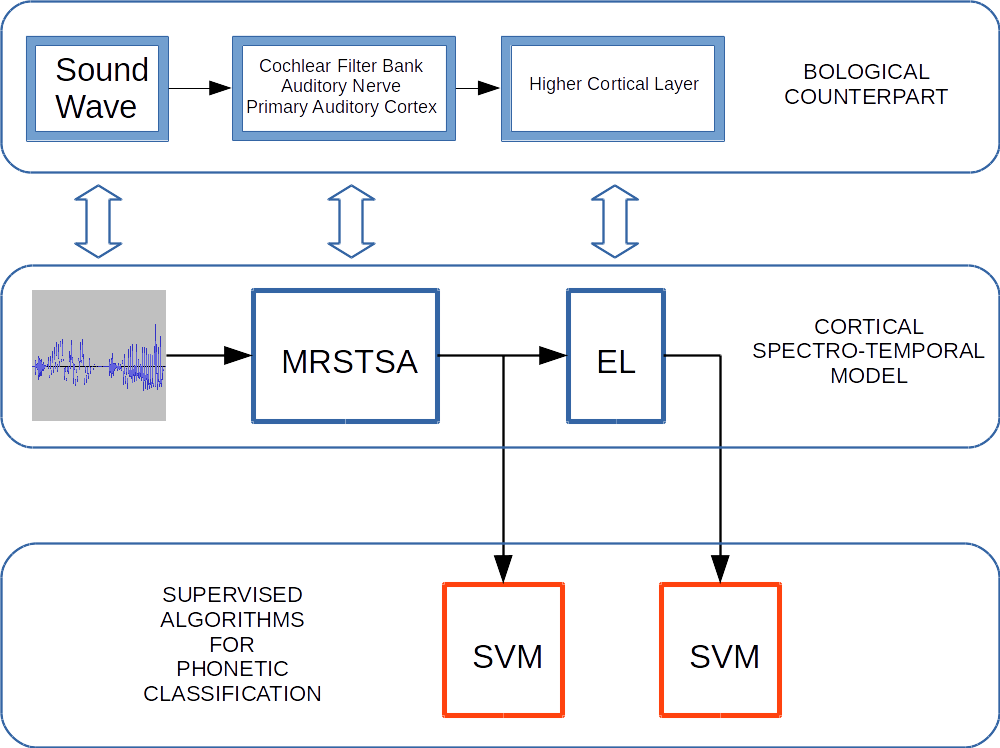
\includegraphics[width=0.8\textwidth]{Experiment.png}
    \caption{Perfil experimental para probar el desempeño en las tareas de clasificación de palabras.
	    Las ondas de sonido son procesadas por el algoritmo \gls{mrstsa}.
    Las salidas desde el \gls{mrstsa} son procesadas por el \gls{el}.
    Las tareas de clasificación de palabras se realizan en ambas salidas por el algpritmo \gls{svm}.
    Cada sección in el \gls{cstm} tiene su contrapartida biológica.}
    \label{fig:Experiment}
\end{figure}



En el procedimiento experimental, primero entrenamos los \glspl{el} diferentes--sección \nameref{model-implementation}--para cada condición silábica. Los \glspl{el}  fueron entrenados utilizando las voces en el primer set y los corpus generados por medio de los métodos descriptos en la sección \nameref{CorpGen}. Luego, procesamos los mismos corpus con los \glspl{el} correspondientes en modo de inferencia. In tal modo, los \glspl{el} procesaron la información con sus propiedades de aprendizaje desabilitadas. De esta forma, durante la inferencia, los \glspl{el} no modificaron sus sinapsis y sólo retornaron patrones de activación en respuesta a los estímulos recibidos. Luego, utilizamos las salidas desde el \gls{mrstsa} y los \glspl{el} en modo de inferencia para entrenar los clasificadores \gls{svm} con el procedimiento explicado en la sección \nameref{model-implementation}. Los desempeños de entrenamiento promedio de validación cruzada se muestran en la Tabla~\ref{SVM_Training}.

\begin{table}[h!]
\centering
\caption{\gls{svm} 5-fold cross validation training results}
\begin{tabular}{|l|l|l|}
\hline
		   & MRSTSA & Encoder Layer \\ \hline
Monosyllabic Words & 99.4\% & 99.52\%          \\ \hline
Disyllabic Words   & 99.3\%   & 99.48\%        \\ \hline
Trisyllabic Words  & 99.5\% & 99.58\%          \\ \hline
\end{tabular}
\label{SVM_Training}
\end{table}

En una segunda etapa, corrimos los \glspl{el} en modo de inferencia, pero esta vez utilizamos corpus diferentes generados utilizando las mismas voces y manipulados con varios tipos de variantes acústicas (ruido balnco, reverberación y variaciones de tono), generadas utilizando el software Audacity. También corrimos los \glspl{el} en modo de inferencia utilizando corpus generados con voces diferentes (el segundo conjunto de voces en sección \nameref{CorpGen}). Testeamos los desempeños de los clasificadores--ya entrenados--frente a las características devueltas por los algoritmos en respuesta a los corpus afectados por las variantes acústicas que introducimos en los nuevos corpus utilizando Audacity \cite{audacity}. Las variantes acústicas introducidas en los nuevos corpus incluyeron ruido blanco, reverberación y variaciones de tono. También probamos los desempeños de clasificación frente a las características devueltas por los algoritmos en respuesta a los nuevos corpus generados con un conjunto diferente de voces.







%In the present work, we studied the level of invariance in the phonetic features abstracted by the \gls{el}, by means of comparing such representations with the multiresolution spectro-temporal auditory features returned by the \gls{mrstsa} algorithm. To this end, we evaluated the features returned by each algorithm in different word classification tasks. \reviewertwo{In order to asses word classification performance} in each algorithm, \reviewertwo{we used the \gls{svm} technique}--section \nameref{model-implementation}--with  the experimental setup depicted in Fig. \ref{fig:Experiment}.

%\begin{figure}[h!]
    %\centering
    %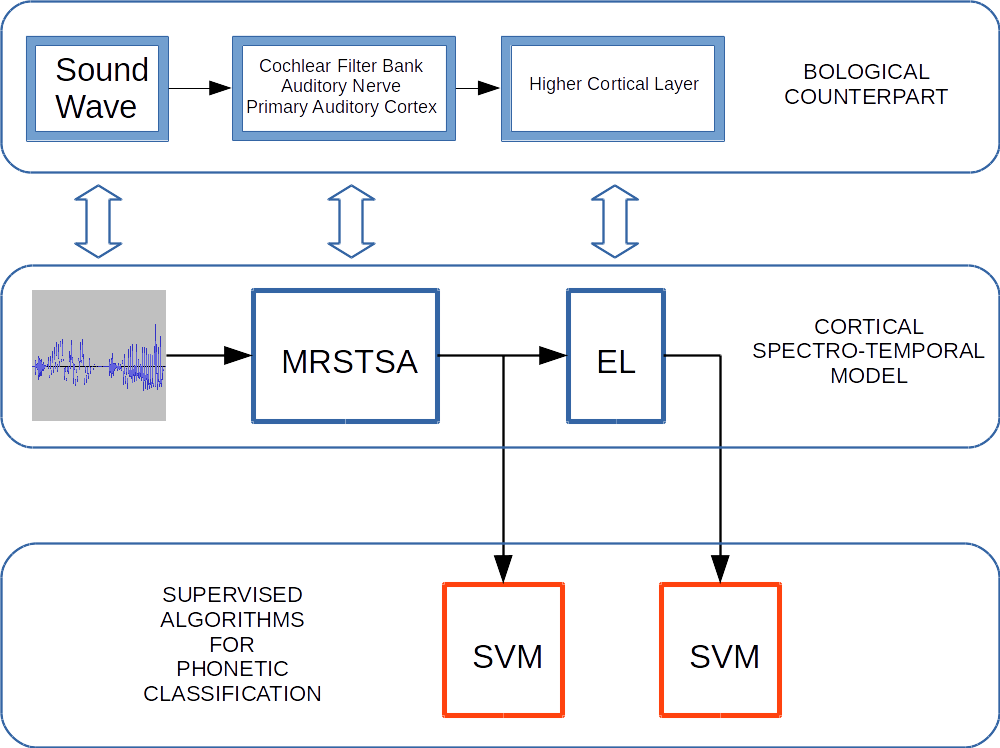
\includegraphics[width=0.8\textwidth]{Experiment.png}
    %\caption{Experimental setup to test word classification task performances.
    %Sound waves are processed by the \gls{mrstsa} algorithm.
    %The outputs from the \gls{mrstsa} are processed by the \gls{el}.
    %Word classification tasks are performed on both outputs by the \gls{svm} algorithm.
    %Each section in the \gls{cstm} has its biological counterpart.}
    %\label{fig:Experiment}
%\end{figure}

%\reviewerfour{In the experimental procedure we first trained 10 different \glspl{el}--section \nameref{model-implementation}--for each syllabic condition. Such \glspl{el} were trained using the voices in set one and the corpora were generated by the method described in section \nameref{CorpGen}. Afterwards, we processed the same corpora with the corresponding \glspl{el} in inference mode. In such mode, the \glspl{el} processed the information with their learning properties disabled. In this manner, during inference, the \glspl{el} did not modify its synapses and just returned patterns of activation in response to the stimuli they received. We then used the outputs from the \gls{mrstsa} and the \glspl{el} in inference mode to train the \gls{svm} classifiers with the procedure depicted in section \nameref{model-implementation}. The average cross validation training performances are shown in Table~\ref{SVM_Training}}.

%\begin{table}[h!]
%\centering
%\caption{\gls{svm} 5-fold cross validation training results}
%\begin{tabular}{|l|l|l|}
%\hline
                   %& MRSTSA & Encoder Layer \\ \hline
%Monosyllabic Words & 99.4\% & 99.52\%          \\ \hline
%Disyllabic Words   & 99.3\%   & 99.48\%        \\ \hline
%Trisyllabic Words  & 99.5\% & 99.58\%          \\ \hline
%\end{tabular}
%\label{SVM_Training}
%\end{table}

%\reviewerfour{In a second stage, we ran the \glspl{el} in inference mode again, but \reviewertwo{this time we used different corpora generated using the same voices and manipulated with several types of acoustic variants (white noise, reverberation and pitch variations), generated using the Audacity software}. We also ran the \glspl{el} in inference mode using corpora generated with different voices (set two voices in section \nameref{CorpGen}). We tested the performances of the--already trained--classifiers in the presence of the features returned by the algorithms in response to the corpora affected by the \reviewertwo{acoustic variants} which we introduced to the new corpora by means of Audacity \cite{audacity}. The \reviewertwo{acoustic variants} introduced to the new corpora included white noise, reverberation and pitch variations. We also tested the classifier performances in the presence of the features returned by the algorithms in response to the new corpora generated with a different set of voices}.




















\section{Resultados}

Los desempeños de clasificación se muestran en la Fig. \ref{fig:PLOT}. 

\begin{figure}[h!]
    \centering
    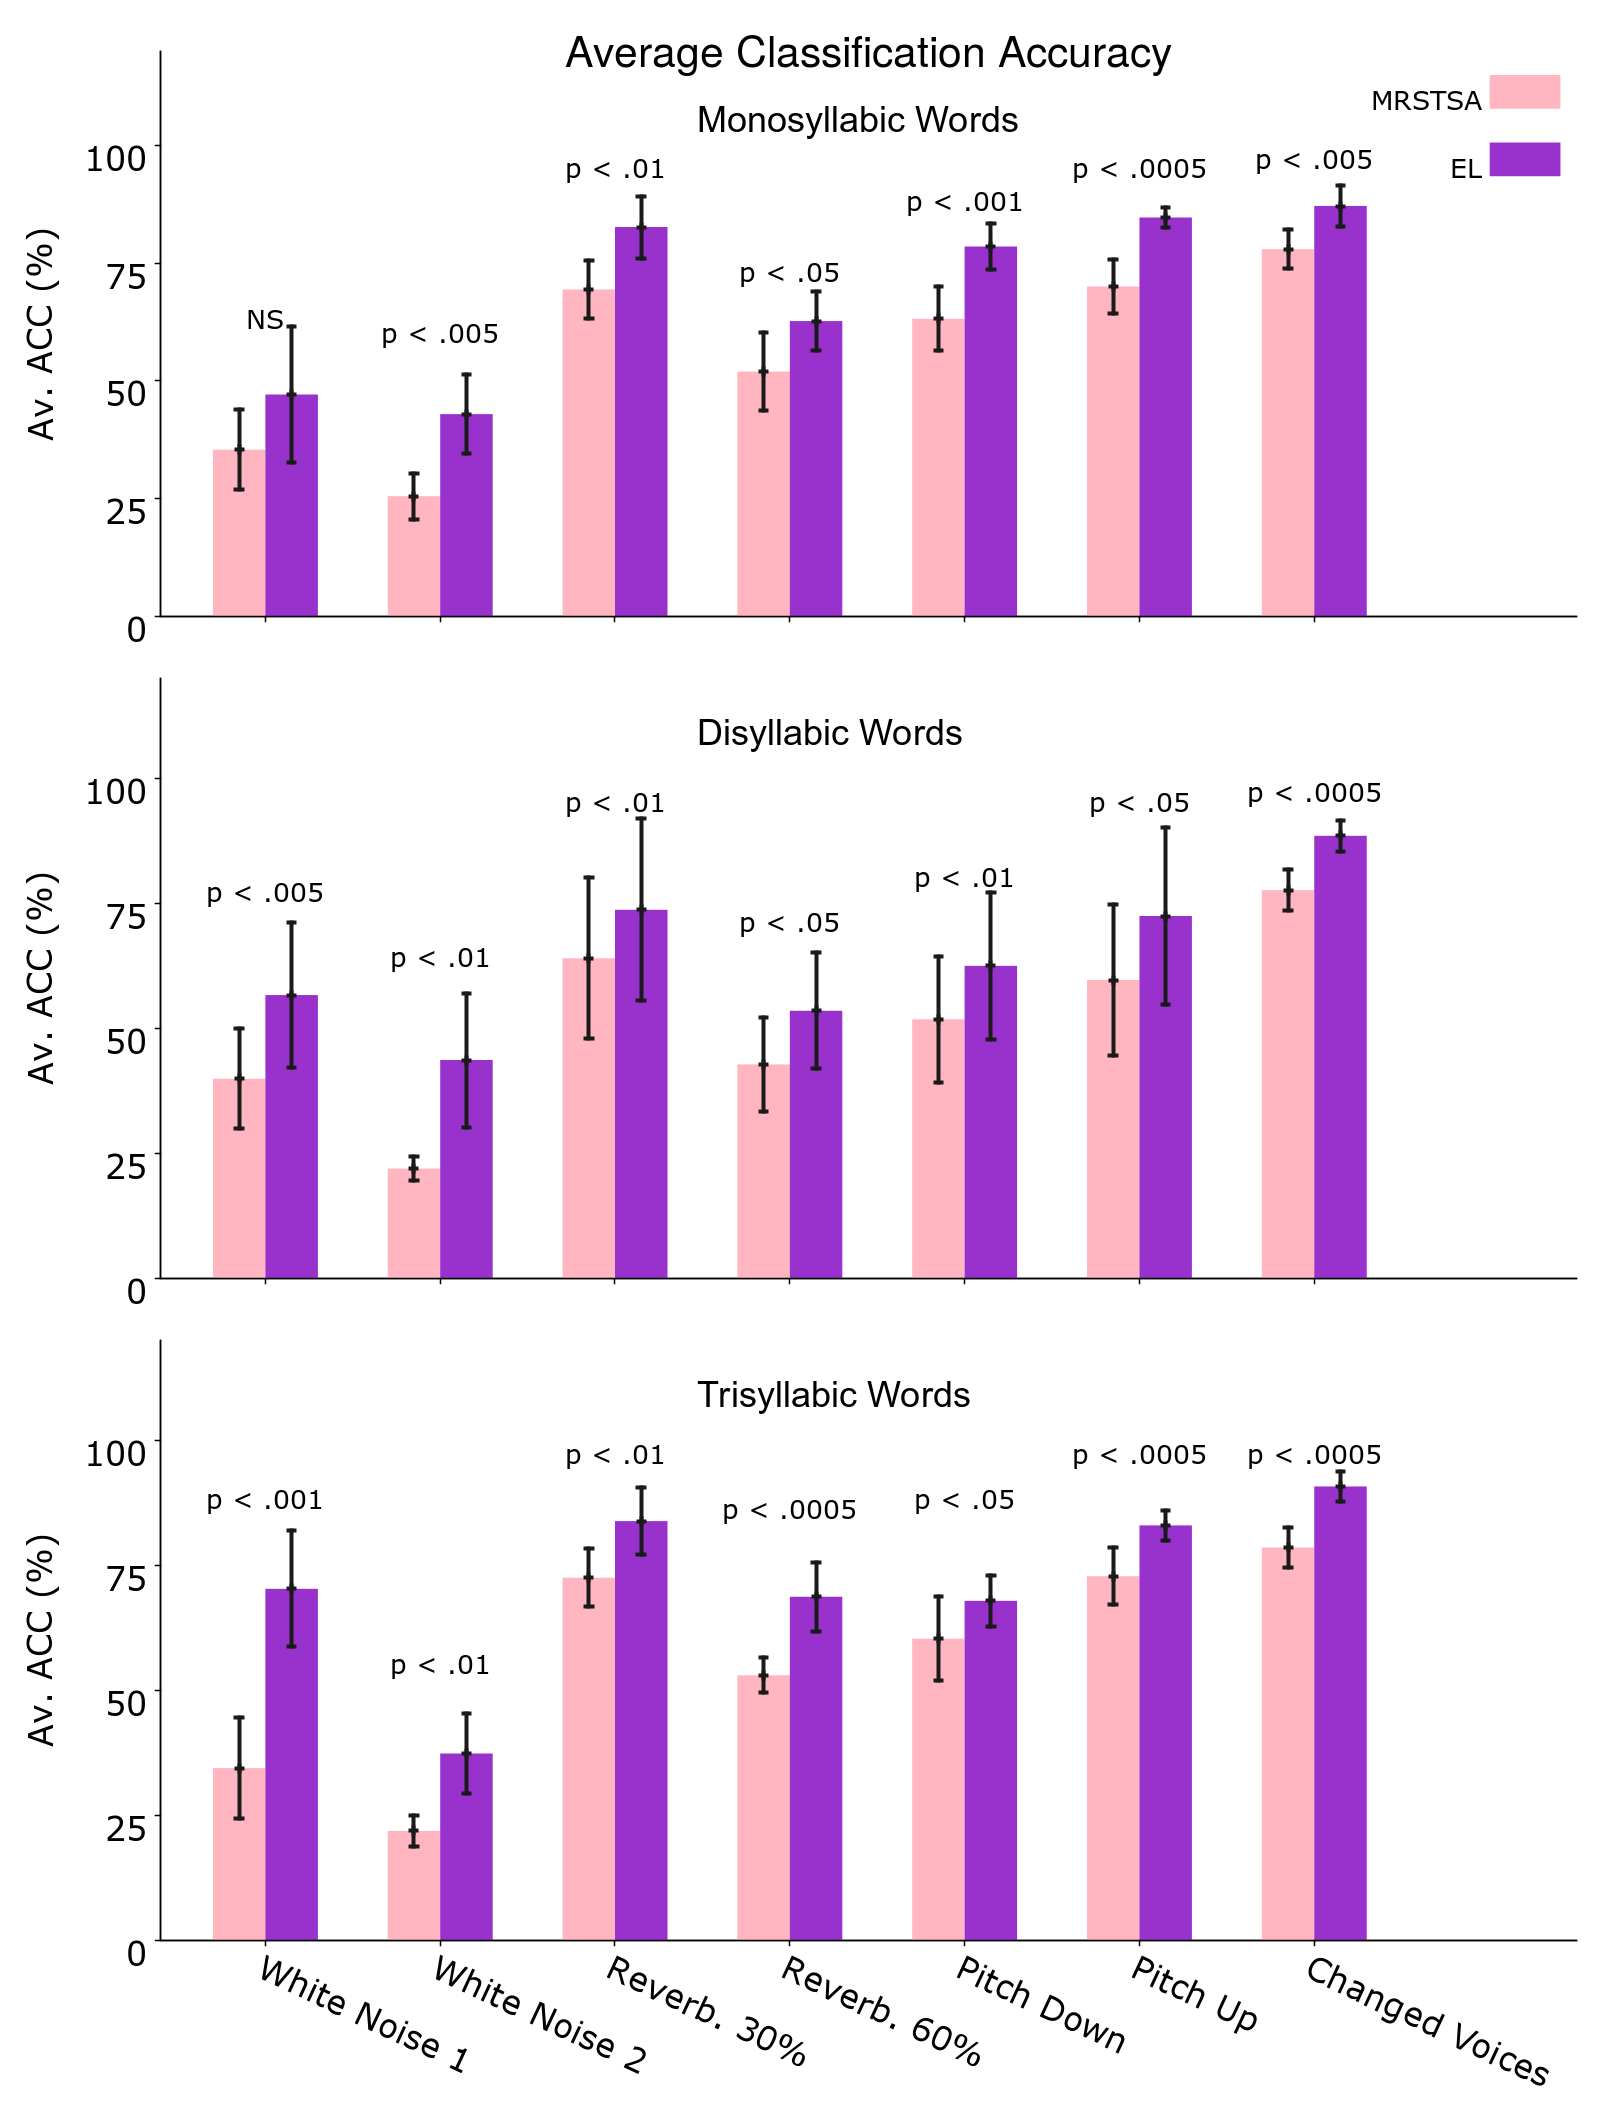
\includegraphics[width=0.8\textwidth]{PLOT.png}
    \caption{Exactitud promedio de clasificación en el \gls{mrstsa} y el \gls{el} frente a differentes variantes acústicas introducidas en las señales para palabras monosilábicas, bisilábicas y trisilábicas.
	    Ruido Blanco 1 determina una \gls{snr} tasa de potencia \gls{rms} promedio de 19.8 dB mientras que Ruido Blanco 2 es de 13.8 dB.
	    Reverberación 30\% determina un valor de \gls{rt} de 0.61 segundos mientras que Reverberación 60\% determina un valor de \gls{rt} de 1.78 segundos.
	    Tono Hacia Arriba determina una corrida de tono desde E hasta G, mientras que Tono Hacia Abajo determina una corrida de tono desde E hasta C. Voces Cambiadas corresponden a los corpus generados utilizando voces diferentes a las voces usadas para entrenar el \gls{el} y los clasificadores. Las barras de error muestran Intervalos de Confianza del 95\%. Los valores de \emph{p} corresponden a t-tests pareados de doble cola y NS intica Estadísticamente no Significativo.}
    \label{fig:PLOT}
\end{figure}

En cuanto al ruido balnco, introducimos ruido blanco aditivo en las señales de los corpus con con una relación de señal a ruido \gls{rms} promedio de tasa de potencia de 19.9 dB (Ruido Blanco 1) y 13.8 dB (Ruido Blanco 2). En cuanto a reverberación, modificamos las señales de los corpus por medio de valores de \gls{rt} de 0.61 segundos (Reverberación 30\%) y 1.78 segundos (Reverberación 60\%). \gls{rt} hace referencia al tiempo que toma una señal para disminuir su amplitud en 60 dBs por debajo de su valor inicial. En cuanto a las variaciones de tono, modificamos los tonos de las señales en los corpus en +20\% (de E a G) (Tono Hacia Arriba) y en -20\% (de E a C) (Tono Hacia Abajo). También utilizamos corpus generados con voces diferentes a las utilizadas para entrenar los \glspl{el} y los \glspl{svm}.

La Fig. \ref{fig:PLOT} muestra la exactitud en clasificación de 5 vías para corpus de palabras monosilábicas, bisilábicas y trisilábicas afectadas por ruido blanco, reverberación y variaciones de tono y voz. Como se puede apreciar en las figuras, el \gls{el} supera al \gls{mrstsa} en todos los casos. Tal comportamiento persiste aún en palabras multisilábicas.

Aplicamos t-tests pareados de doble cola para los 10 diferentes corpus generados con los 10 vocabularios diferentes--sección \nameref{CorpGen}. Como se puede ver en la Fig. \ref{fig:PLOT}--exepto para palabras monosilábicas con Ruido Blanco 1 $(p < 0.22)$--obtuvimos significación estadística para todas las condiciones considerando $(p<0.05)$. 
Dado que se llevaron a cabo 7 t-tests para cada tarea de clasificación de palabras independiente (por ejemplo, palabras monosilábicas, bisilábicas y trisilábicas), aplicamos correcciónes de Holm-Bonferroni con un factor de corrección de 7 a los fines de reducir la probabilidad de errores de tipo I y de tipo II en el contexto de las diferentes condiciones experimentales \cite{10.1093/biomet/75.2.383}. Por medio de tales correcciones confirmamos la significación estadística para todos los casos mostrados en la Fig. \ref{fig:PLOT}.

La Fig. \ref{fig:PLOT1} muestra la exactitud de clasificación promedio para todas las variantes acusticas para palabras mono, bi y trisilábicas.
En este caso, también realizamos t-tests pareados de doble cola, pero esta vez para 7 condiciones de variantes acústicas difernetes.
Como se puede apreciar en la figura, todas la pruebas realizadas fueron estadísticamente significativas  y la capa del encoder muestra una clara y sostenida superioridad para palabras con un número diferente de sílabas.

\begin{figure}[h!]
    \centering
    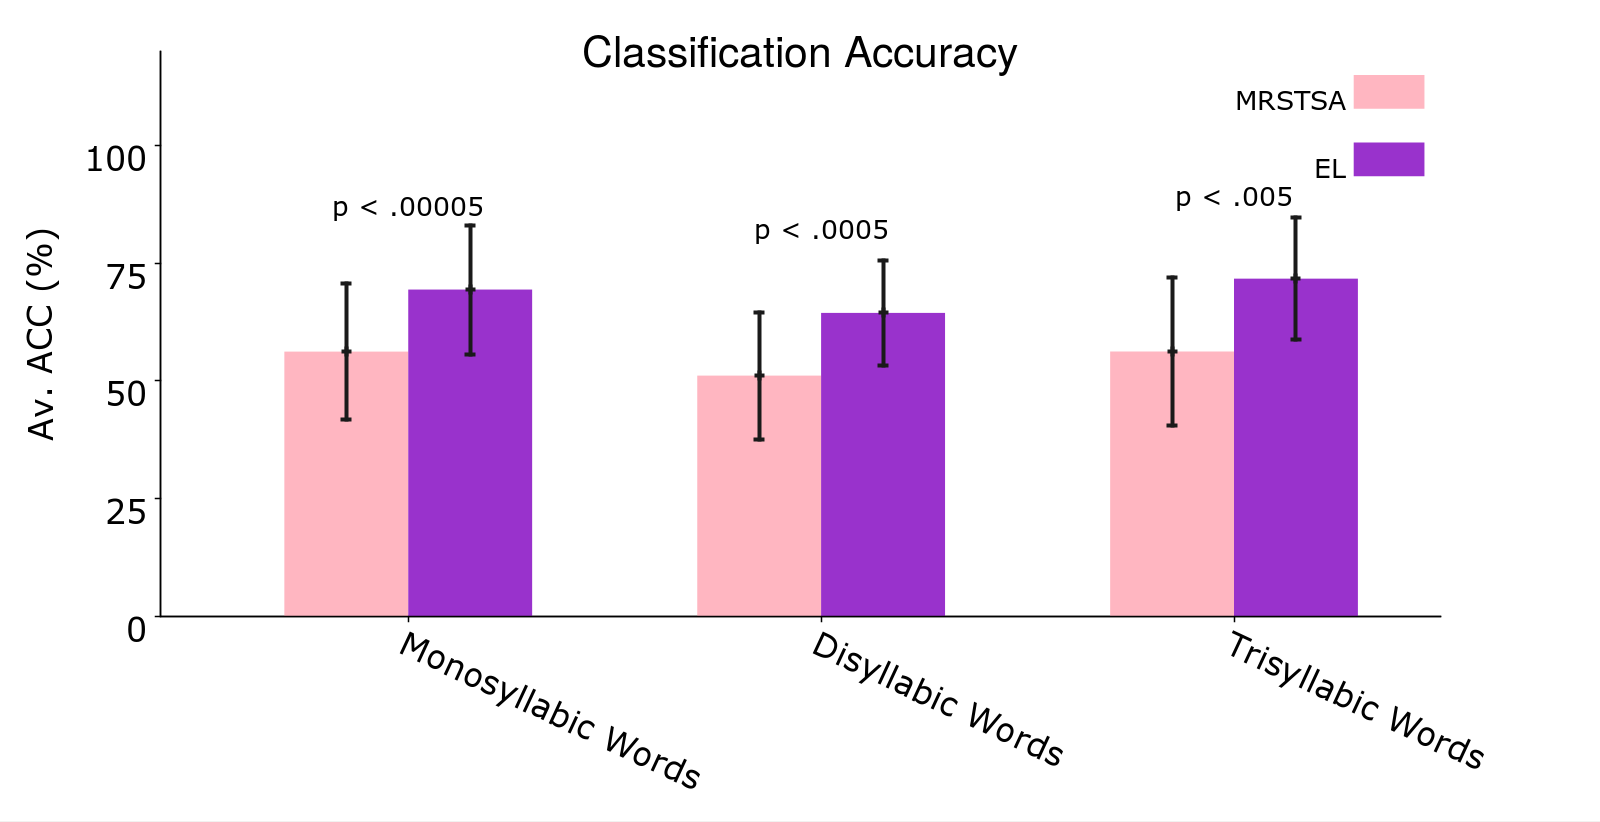
\includegraphics[width=0.8\textwidth]{PLOT1.png}
    \caption{Exactitud en clasificación promedio a través de todas las variantes acústicas para palabras mono, bi y trisilábicas. Las barras de error exhiben un Intérvalo de Confianza del 95\%. Los valores de \emph{p} corresponden a t-tests pareados de doble cola.}
    \label{fig:PLOT1}
\end{figure}


%The classification performances are shown in Fig. \ref{fig:PLOT}.

%\begin{figure}[h!]
    %\centering
    %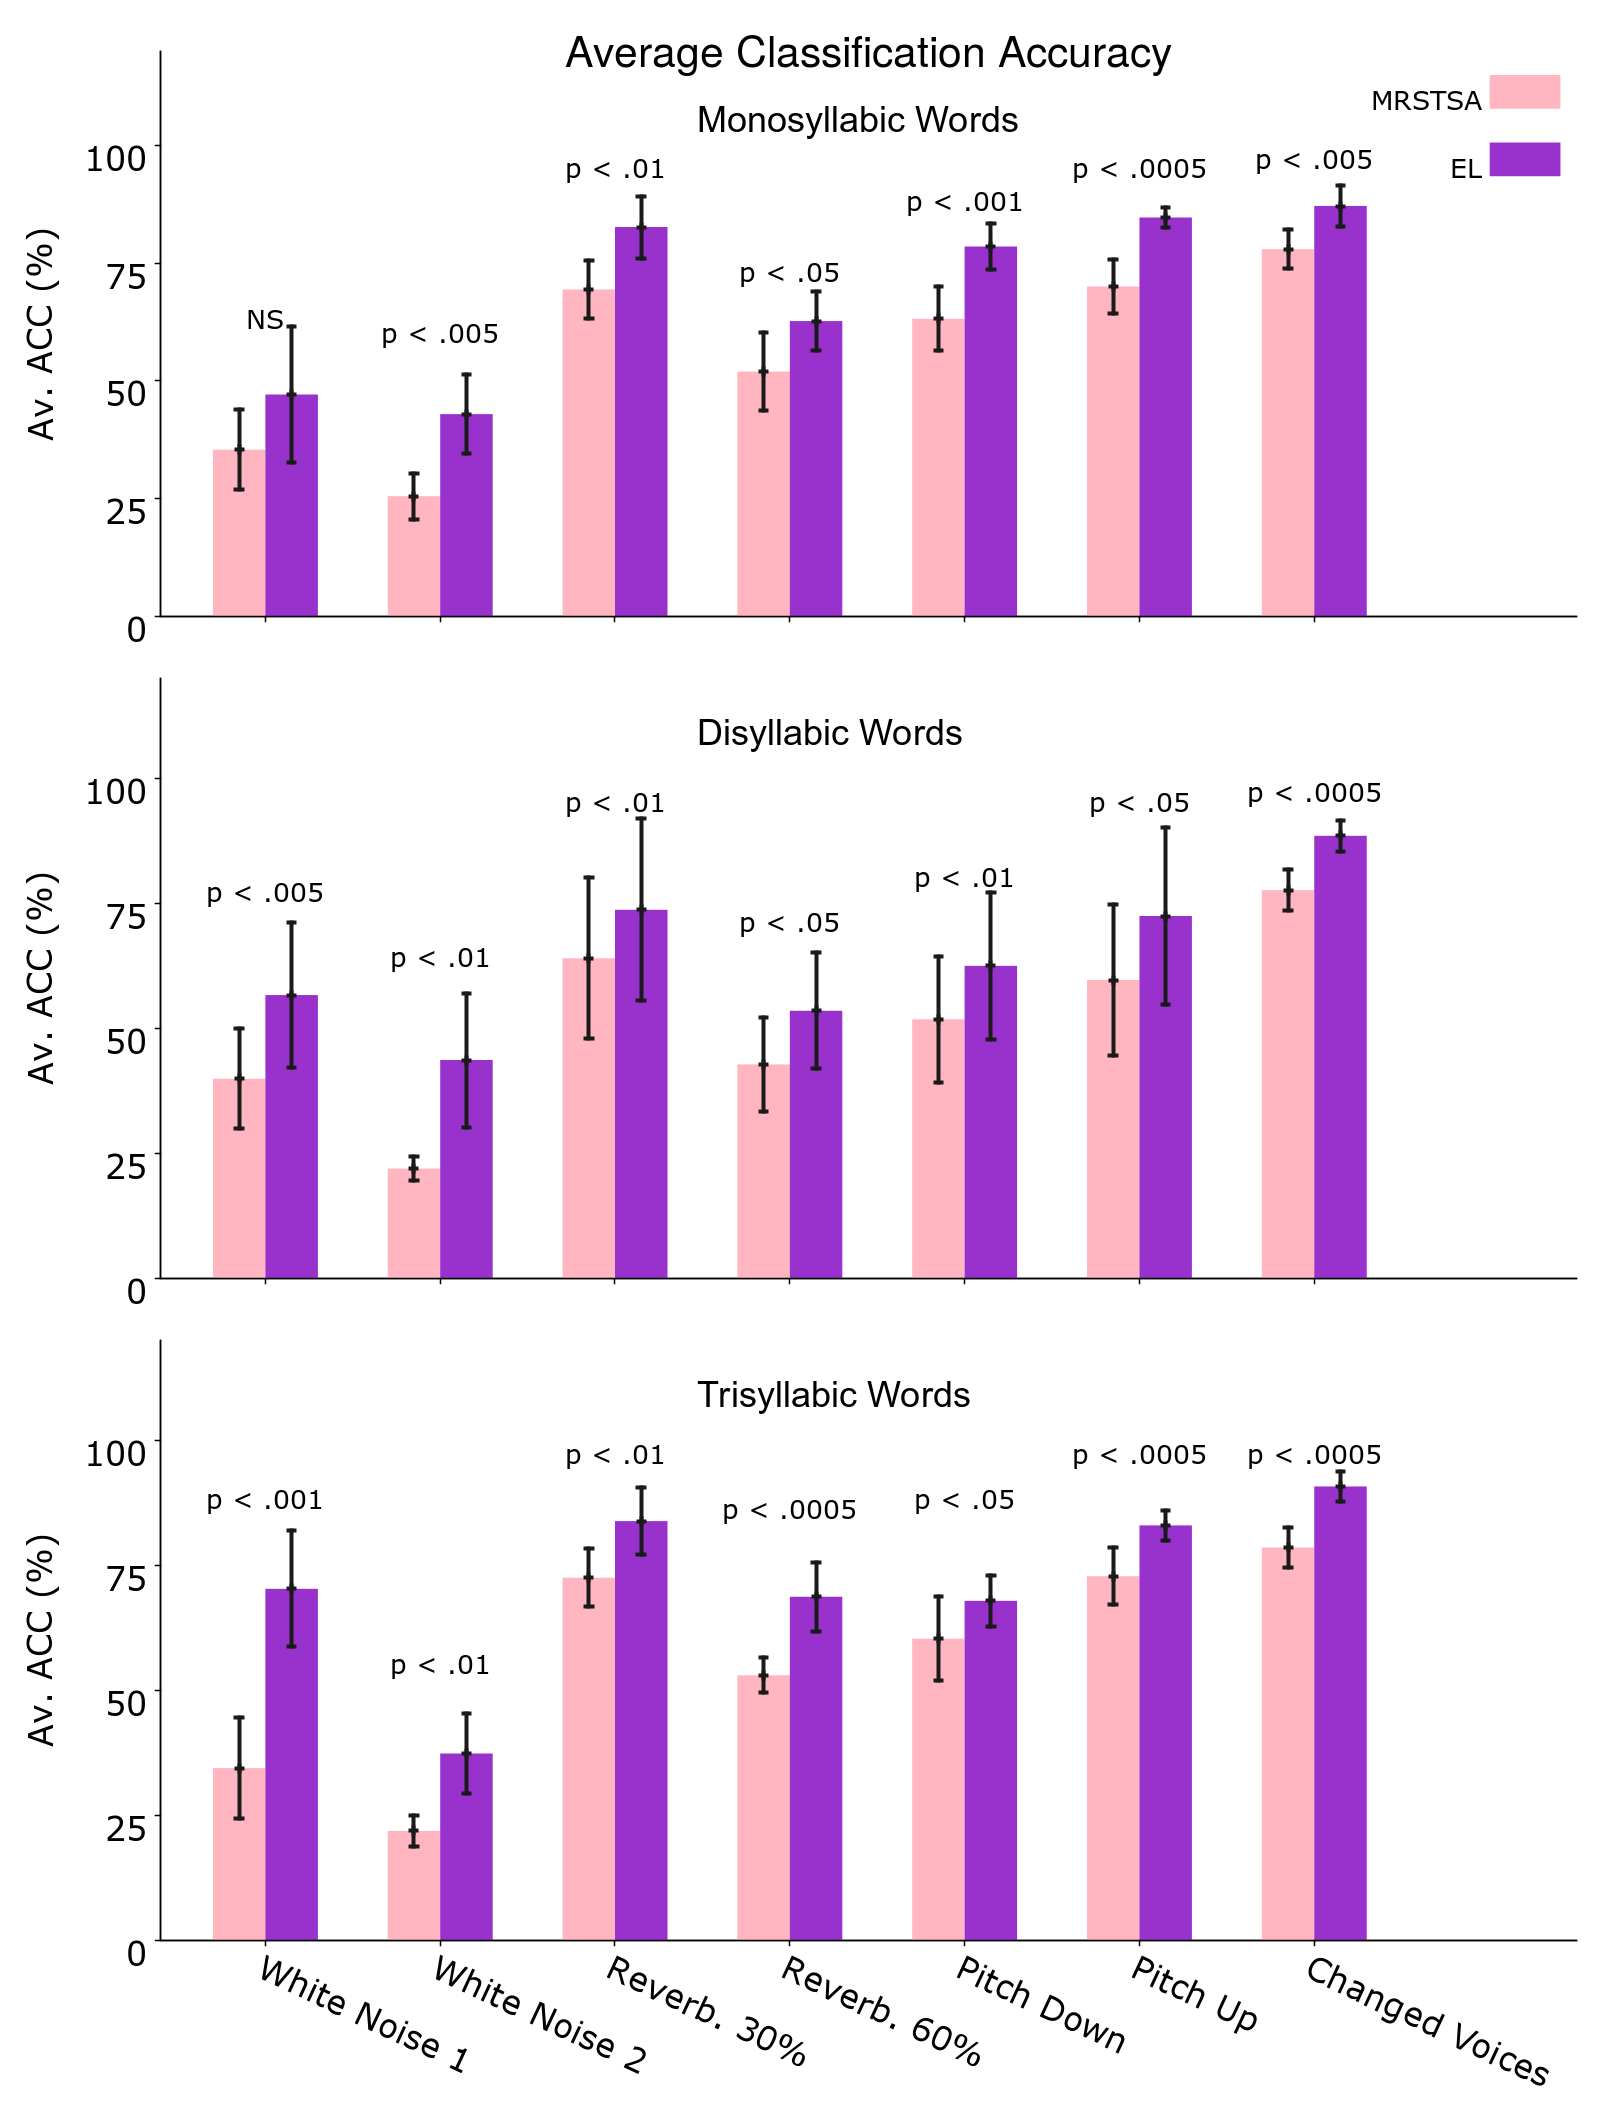
\includegraphics[width=0.9\textwidth]{PLOT.png}
    %\caption{\gls{mrstsa} and \gls{el} average classification accuracies against different \reviewertwo{acoustic variants} introduced to the signals
    %for monosyllabic, disyllabic and trisyllabic words.
    %White Noise 1 determines a \gls{snr} average \gls{rms} power rate of 19.8 dB while White Noise 2 13.8 dB.
    %Reverberation 30\% determines a \gls{rt} value of 0.61 seconds while Reverberation 60\% determines a \gls{rt} value of 1.78 seconds.
    %Pitch Up determines a pitch move from E to G, while Pitch Down determines a pitch move from E to C. Changed Voices corresponds to corpora generated using a different set of voices from the one used to train the \glspl{el} and the classifiers. \reviewertwo{Error bars depict 95\% Confidence Interval values. The \emph{p} values correspond to \newreview{two-tailed} paired t-tests and NS stands for Not Statistically Significant.}}
    %\label{fig:PLOT}
%\end{figure}

%%\begin{figure}[h!]
    %%\centering
    %%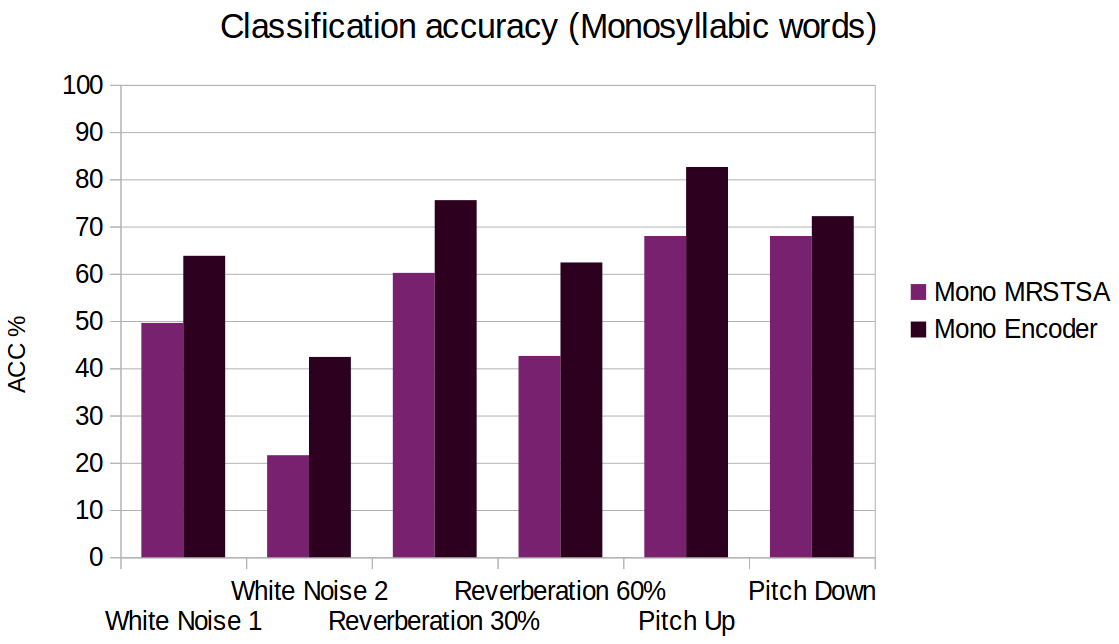
\includegraphics[width=0.9\textwidth]{MONO_ACC.png}
    %%\caption{\gls{mrstsa} and \gls{el} classification accuracies against different \reviewertwo{acoustic variants} introduced to the original signals
    %%for \textbf{monosyllabic words}.
    %%White Noise 1 determines a \gls{snr} average \gls{rms} power rate of 19.8 dB while White Noise 2 13.8 dB.
    %%Reverberation 30\% determines a \gls{rt} value of 0.61 seconds while Reverberation 60\% determines a \gls{rt} value of 1.78 seconds.
    %%Pitch Up determines a pitch move from E to G, while Pitch Down determines a pitch move from E to C.}
    %%\label{fig:MONO_ACC}
%%\end{figure}

%%\begin{figure}[h!]
    %%\centering
    %%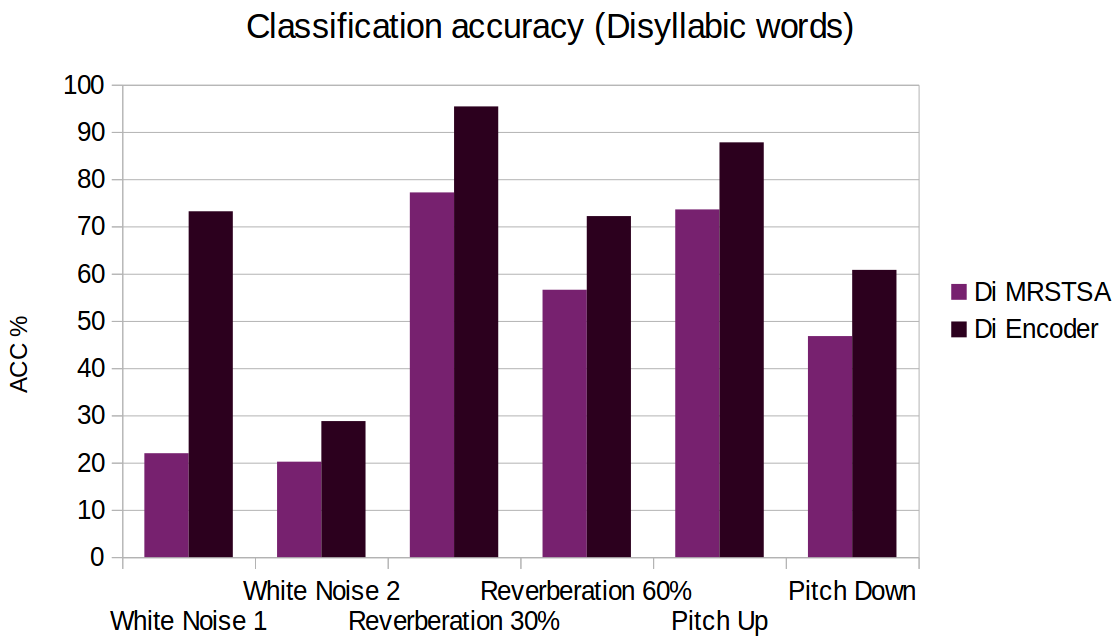
\includegraphics[width=0.9\textwidth]{DI_ACC.png}
    %%\caption{\gls{mrstsa} and \gls{el} classification accuracies against different \reviewertwo{acoustic variants} introduced to the original signals
    %%for \textbf{disyllabic words}.
    %%White Noise 1 determines a \gls{snr} average \gls{rms} power rate of 19.8 dB while White Noise 2 13.8 dB.
    %%Reverberation 30\% determines a \gls{rt} value of 0.61 seconds while Reverberation 60\% determines a \gls{rt} value of 1.78 seconds.
    %%Pitch Up determines a pitch move from E to G, while Pitch Down determines a pitch move from E to C.}
    %%\label{fig:DI_ACC}
%%\end{figure}

%%\begin{figure}[h!]
    %%\centering
    %%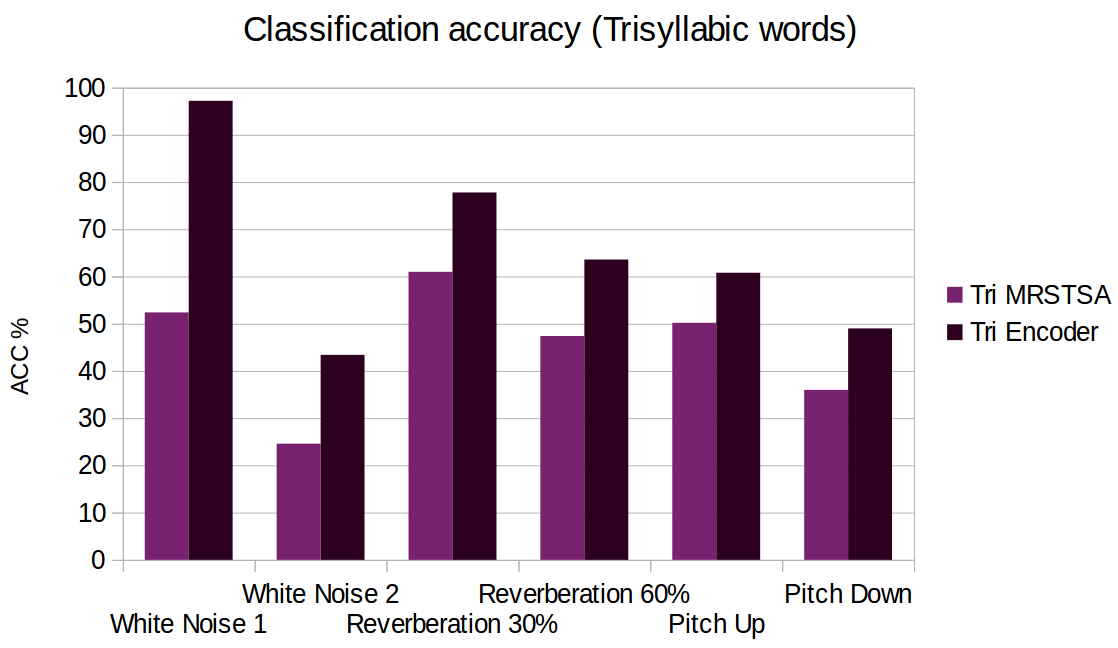
\includegraphics[width=0.9\textwidth]{TRI_ACC.png}
    %%\caption{\gls{mrstsa} and \gls{el} classification accuracies against different \reviewertwo{acoustic variants} introduced to the original signals
    %%for \textbf{trisyllabic words}.
    %%White Noise 1 determines a \gls{snr} average \gls{rms} power rate of 19.8 dB while White Noise 2 13.8 dB.
    %%Reverberation 30\% determines a \gls{rt} value of 0.61 seconds while Reverberation 60\% determines a \gls{rt} value of 1.78 seconds.
    %%Pitch Up determines a pitch move from E to G, while Pitch Down determines a pitch move from E to C.}
    %%\label{fig:TRI_ACC}
%%\end{figure}

%%\pagebreak

%Regarding white noise, we introduced additive white noise to the corpora signals with signal-noise average \gls{rms} power rate of 19.9 dB (White Noise 1) and 13.8 dB (White Noise 2). In terms of reverberation, we modified the corpora signals by means of \gls{rt} values of 0.61 seconds (Reverberation 30\%) and 1.78 seconds (Reverberation 60\%). \gls{rt} Is the time that a signal takes to decrease its amplitude to 60 dBs under its initial value. As regards pitch variations, we modified the corpora signals pitch in +20\% (from E to G) (Pitch Up) and in--20\% (from E to C) (Pitch Down). \reviewerfour{We also used corpora generated with different voices from the ones used to train the \glspl{el} and the \glspl{svm}}.

%\iffalse
%\begin{figure}[h!]
    %\centering
    %\includegraphics[width=0.9\textwidth]{Classification.png}
    %\caption{\gls{mrstsa} and \gls{el} classification performances against different \reviewertwo{acoustic variants} introduced to the original signals.
    %Mono means monosyllabic words, Di means disyllabic words and Tri means trisyllabic words.
    %White Noise 1 determines a \gls{snr} average \gls{rms} power rate of 19.8 dB while White Noise 2 13.8 dB.
    %Reverberation 30\% determines a \gls{rt} value of 0.61 seconds while Reverberation 60\% determines a \gls{rt} values of 1.78 seconds.
    %Pitch Up determines a pitch move from E to G, while Pitch Down determines a pitch move from E to C.}
    %\label{fig:Classification}
%\end{figure}
%\fi


%Fig. \ref{fig:PLOT}
%\reviewertwo{shows a 5-way word classification accuracy} for mono, di and trisyllabic word corpora affected by
%white noise, reverberation and pitch \reviewerfour{and voice} variations.
%As can be seen in the figures, the \gls{el} outperforms the \gls{mrstsa} in all cases.
%Such behavior persists for multisyllabic words.

%\reviewertwo{We performed \newreview{two-tailed} paired t-tests for 10 different corpora generated from 10 different vocabularies--section \nameref{CorpGen}. As can be seen in Fig. \ref{fig:PLOT}--except for monosyllabic words with White Noise 1 \newreview{$(p < 0.22)$}--there was Statistical Significance for all conditions considering $(p<0.05)$}.

%\newreview{Given that we conducted 7 t-tests for each independent word classification task (i.e. mono, di and trisyllabic words), we performed Holm–Bonferroni corrections with a correction factor of 7 in order to reduce the probability of type I and type II errors in the context of the different experimental conditions \cite{10.1093/biomet/75.2.383}. By means of such corrections we confirmed the statistical significance for all the cases showed in Fig.\ref{fig:PLOT}.}

%Fig. \ref{fig:AV_ACC} shows average classification accuracies across all \reviewertwo{acoustic variants} for mono, di and trisyllabic words.
%\reviewertwo{In this case, we also performed \newreview{two-tailed} paired t-tests, but this time for 7 different acoustic variant conditions.
%As can be seen in the figure, all performed tests are statistically significant and the encoder layer clearly shows
%a sustained superiority across words with different number of syllables}.
 

%\begin{figure}[h!]
    %\centering
    %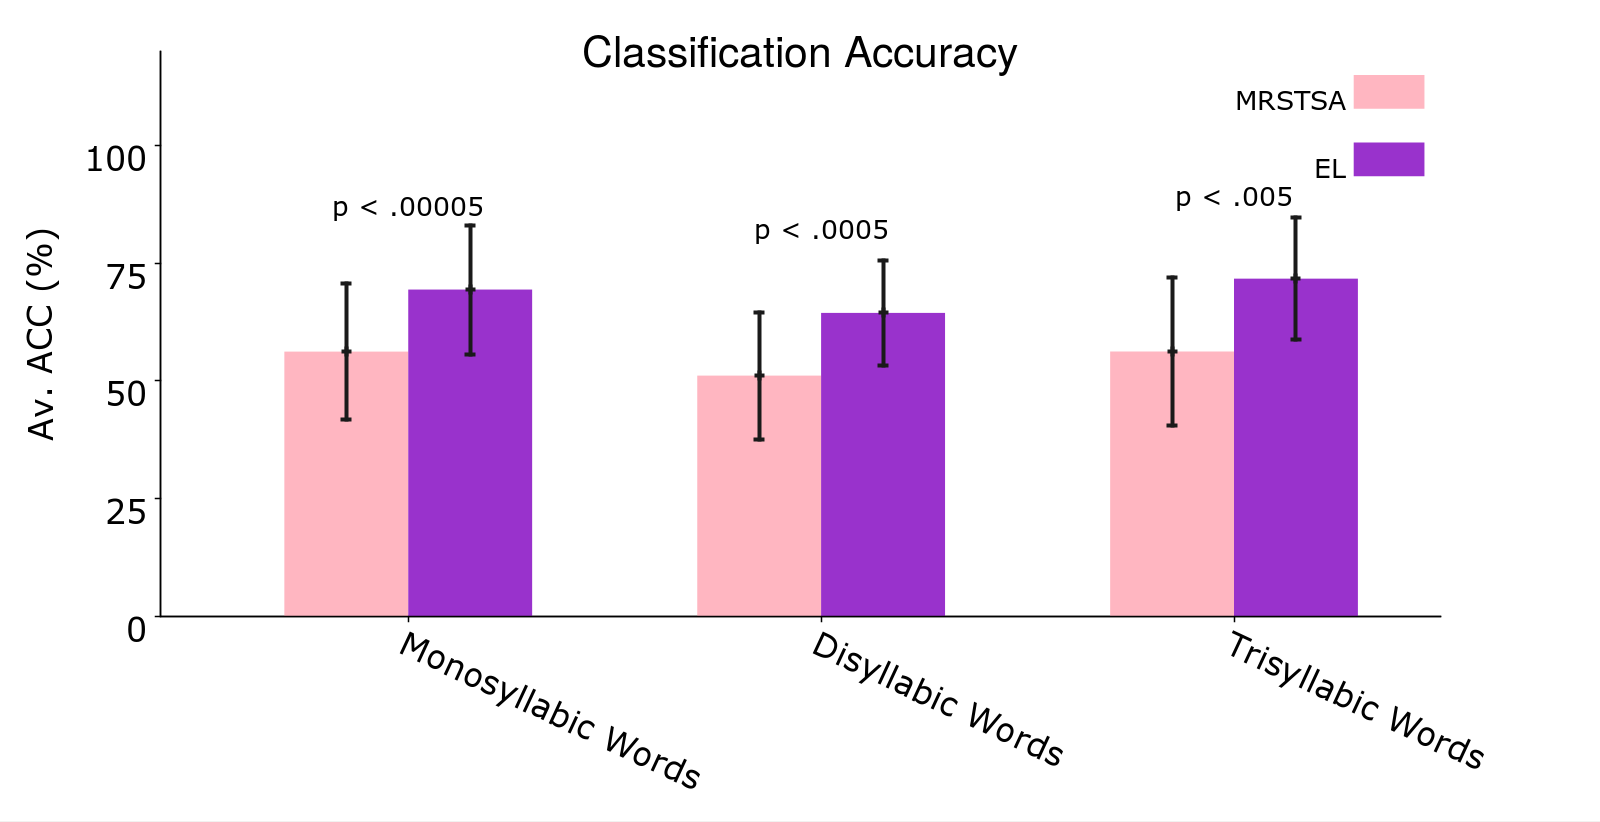
\includegraphics[width=0.9\textwidth]{PLOT1.png}
    %\caption{Average classification accuracies across all \reviewertwo{acoustic variants} for mono, di and trisyllabic words. \reviewertwo{Error bars depict 95\% Confidence Interval values. The \emph{p} values correspond to \newreview{two-tailed} paired t-tests}.}
    %\label{fig:AV_ACC}
%\end{figure}

%%\begin{figure}[h!]
    %%\centering
    %%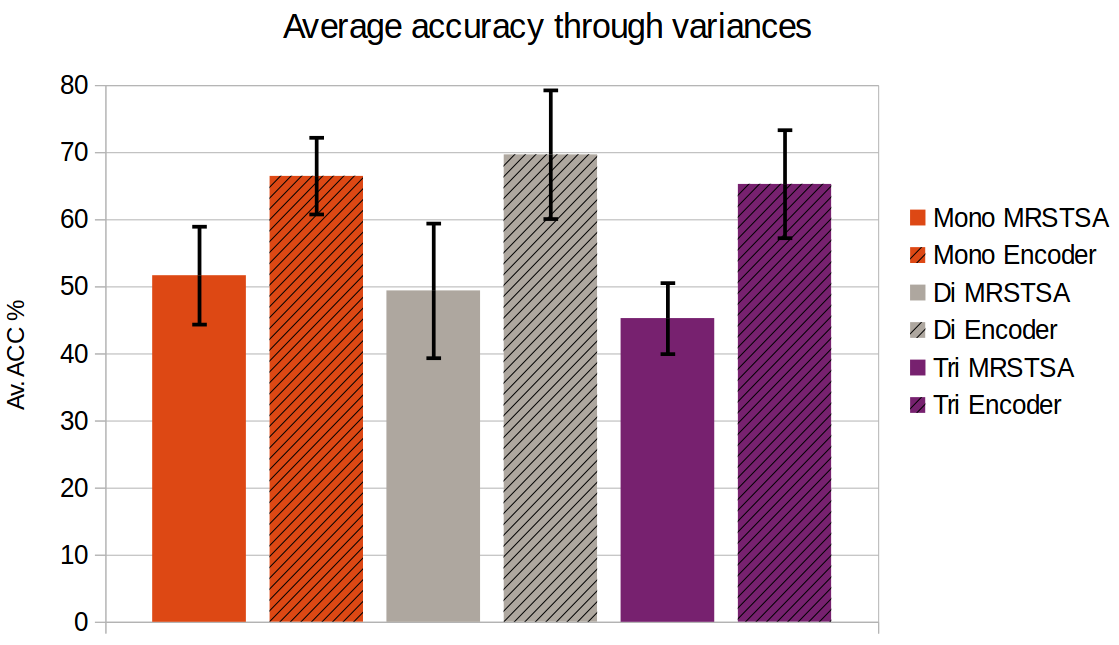
\includegraphics[width=0.9\textwidth]{AV_ACC.png}
    %%\caption{Average classification accuracies across all \reviewertwo{acoustic variants} for mono, di and trisyllabic words with Standard Error bars.
    %%Mono means monosyllabic words, Di means disyllabic words and Tri means trisyllabic words.}
    %%\label{fig:AV_ACC}
%%\end{figure}















\section{Discusión}

Los resultados obtenidos en este trabajo sostienen las hipótesis computacionales propuestas en nuestro enfoque de modelaje para imitar invarianza y generalización fonética incidental.
ALgunas de las hipótesis ya han sido explicadas en términos de sus propiedades  \cite{hawkins_2016}, pero más específicamente, en términos de sus capacidad de aprendizaje de secuencias \cite{cui_2016}.
Des todas maneras, no existen precedentes de tales características neurofisiológicas probadas en tareas de clasificación como las que se llevan acabo en el presente trabajo, en las que reglas fonotácticas se adquieren sin la aplicación de procedimientos de obtimización como tal como la propagando arrores acia atrás por medio de descenso de gradiente. Adicionalmente, nuestro enfoque presenta diferencias sustanciales en términos de sus características de implementación algorítmica. En este trabajo, las sinápsis distantes proveen contribuciones individuales y nuestra organización anatómica micro-columnar adquiere su comportamiento fisiológico espontaneamente con el aprendizaje. También probamos tales características en una realización con cientos de columnas corticales cada una combinando varias micro-columnas con activaciones aferentes estocásticas cuyas futuras implementaciones estás destinadas a explorar simulaciones a gran escala en sistemas computacionales de desempeño lideres a nivel mundial.

Algunos modelos computacionales han sido desarrollados previamente para entender como categorías fonéticas son adquisidas~\cite{rasanen_2012}. El objetivo en dichos trabajos ha sido principalmente explicar aspectos relevantes de la adquisición fonética, sin dar detalles en cuanto a cómo el cerebro podría proveer tales computaciones.
Lee et al. (2009), empleó aprendizaje no supervisado para clasificación de audio con \glspl{cdbn}~\cite{Lee:2009:UFL:2984093.2984217}. 
Los autores probaron el desempeño en clasificación de un modelo con dos capas en la exactitud de una tarea de clasificación de phonemas en 39 vías sobre el dataset \gls{timit} para varios números de oraciones de entrenamiento. 
La primera capa nunca superó el algoritmo \gls{mfcc} que fue utilizado como entrada a la red.
Es más, en tal trabajo no se reportó el desempeño de la segunda capa ya que esta no pudo superar a la primera.
El máximo desempeño reportado para la primer capa fue 64.4\% contra un desempeño del 79.6\% para el \gls{mfcc}.
Sólo fue posible reportar un desempeño del 80.3\% combinando ambos, el \gls{mfcc} y la primer capa en la \gls{cdbn}.

En un trabajo más reciente, la capacidad de \glspl{dmn}--una modificación de arquitectura \glspl{dnn} alimentada en directo que utiliza la función de activación max-out--para manejar ruido ambiental fue investigada frente a diferentes clases fonéticas y para diferentes condiciones de ruido \cite{silos_2016}. En tales experimentos--con la excepción de fonemas fricativos para 15 dB \gls{snr} de Ruido Callejero--el desempeño nunca superó el 70\%. Es más, el desempeño se vio seriamente deteriorado en presencia de ruido blanco de 15 dB \gls{snr}, resultando en una exactitud de clasificación bien por debajo del 60\% in todos los casos.

En el trabajo aquí presentado, reportamos desempeños en clasificación de--por ejemplo--90.8\% para el \gls{el} contra 78.58\% para el \gls{mrstsa} para palabras trisilábicas frente a voces cambiadas (es decir, voces que nunca fueron "oidas" por el \gls{el} durante el entrenamiento; Fig. \ref{fig:PLOT}), también reportamos desempeños por encima del 70\% en el \gls{el} contra un desempeño por debajo del 35\% en el \gls{mrstsa} para palabras trisilábicas frente a ruido blanco de 19.8dB \gls{snr} y desempeños bien arribade 40\% para palabras mono y bisilábicas frente a ruido blanco de 13.8 dB \gls{snr} (Fig. \ref{fig:PLOT}). También reportamos que el \gls{el} superó al \gls{mrstsa} para todas las condiciones de prueba y que tal comportamiento se sostuvo para diferentes números de sílabas en las palabras utilizando pruebas de significación estadística (Fig. \ref{fig:PLOT1}).

Aunque este es un buen escenario, debemos de ser cuidadosos ya que no podemos ignorar diferencias experimentales imporatantes con respecto a los resultados arrojados por los trabjos previos. Primero, nuestro material de entrenamiento es muy diferente  al utilizado en trabajos previos. Nosotros utilizamos corpus generados por sintetizadores de vos en lugar de corpus estandarizados como \gls{timit}.
Nuestro principal objetivo fue el de replicar adquisición fonética temprana en humanos, lo cual es logrado incidentalmente por infantes \cite{Saffran1996StatisticalLB}.
Dada la buena calidad de las voces sintetizadas por \gls{festival}  \cite{festival2014} y su flexibilidad para componer diferentes tipos de corpus--aún con palabras que no existen en ningún lenguaje--consideramos apropiada su utilización como procedimiento experimental inicial para probar nustro enfoque en un contexto de reglas fonotácticas adquiridas incidentalmente.
Segundo, en este trabajo abordamos tareas de clasificación de palabras multililábicas en contraste con los experimentos de clasificación de fonemas llevados a cabo por las investigaciones previas, ya que estamos principalmente motivados a probar las capacidades de la dinámica secuencial de nuestro modelo para adquirir las reglas fonotácticas detras de los vocabularios de entrenamiento.
Finalmente, reportamos resultados de tareas de clasificación de 5 vías en contraste con tareas de clsificación de 39 vías en \cite{Lee:2009:UFL:2984093.2984217}.
Por un lado, esta última diferencia podría haber actuado en favor de nuestro enfoque considerando que es más facil clasificar una categoría entre 5 que una entre 39.
Por otro lado, es importante resaltar que los trabajos previos han estado provistos de más material de entrenamiento con más vocabularios, más hablantes, etc.
En nuestro caso, presentamos condiciones de entrenamiento más duras, ya que nuestro modelo fuen entrenado con 500 palabras desde un vacabulario de solo 5 palabras pronunciadas por 10 voces.
Más allá del tamaño pequeño de la muestra, el desempeño demostrado por nuestro modelo computacional exhibe niveles significativos de generalización fonética con la capacidad de adquirir reglas fonotácticas y de generalizar a contextos ambientales novedosos. El nuestro e un escenario mucho más biológicammente preciso que aquellos establecidos por otros enfoques in los cuqles sus modelos son entrenados utilizando millones de ejemplos. Nuestro modelo, por lo tanto, imita resultados experimentales que muestran como infantes de 8 meses de edad adquieren las reglas fonotácticas inmersas el el flujo auditivo de entrada con sólo 2 minutos de exposición (180 palabras en total, de un vacabulario de 4 palabras de tres sílabas) \cite{Saffran1996StatisticalLB}.

Somos conscientes que se necesitarán mas pruebas--en diferentes escenarios--con corpus diferentes y estandardizados (como \gls{timit}) para analizar más profundamente las capacidades de nuestro enfoque.
Sin embargo, nuestro objetivo principal en el presente trabajo fue el de probar la invarianza fonética secuencial exhibida por el \gls{el} bajo condiciones experimentales estrictamente controladas en las que se conocieron los niveles de ruio, reverberación y variaciones de tono con los que el estímulo se afectó de manera precisa. El material de entrenamiento para el \gls{el} solo involucró los corpus originales de 500 palabras, pero lo más importante es que el \gls{el} nunca fue espuesto--durante su entrenamiento--a los disturbios utilizados para probar el desempeño de su clsificación. El perfil experimental aplicado en este trabajo (Fig. \ref{fig:Experiment}) deja en claro que el \gls{el} es integramente no supervisado y que toda la supervisión se limita a los algoritmos de \gls{svm}. Es más, el \gls{el} no optimiza la actualización de sus pesos sinápticos utilizando descenso del gradiente propagando errores producidos por funciones de costo arbitrariamente insertadas. Este es un punto fundamental para demostrar la plausibilidad biológica de nuestra implementación ya que las restricciones fonotácticas en los  lenguajes humanos son adquiridas incidentalmente \cite{BRENT199693,saffran_1997} y por lo taanto, supervisión alguna se podría tolerar bajo tales circunstancias comportamentales.

En futuras investigaciones propiedades dinámicas emergentes podrían surgir de la incorpoaración de capas corticales subsecuentes--más allá del \glsfirst{el}--en los pasos de procesamiento del modelo. De esta forma podremos implementar dendritas apicales distantes hacia atrás las cuales traerán contexto por medio de una implementación jerárquica no supervisada.
Aunque tal retroalimentación podría ser útil en el contexto de la adquisición fonética insidental, el modelado de la competencia fonética adulta podría posiblemente requerir la implementación de hipótesis más complejas para nuestro modelo. La incorporación de funciones de costo con más precisión biológica para poder retroalimentar cualquier tipo de error de activación requerirá hipótesis biológicamente precisas. ¿Deberían esos errores ser señales escalares (mecanismos de refuerzo) o deberían ser vectores (mecanismos supervisados)? ¿Deberían de venir desde la misma modalidad o deberían ser traidas desde una modalidade diferente? ¿Deberían variar a través de parches corticales diferentes o deberían variar durante el desarrollo temporal? \cite{10.3389/fncom.2016.00094}.
Un mecanismo supervisado asistido por diferentes areas corticales de forma multimodal podría ser una hipótesis biológicamente precisa ya que se ha mostrado como gestos icónicos impulsan la comprensión del habla bajo condiciones auditivas adversas \cite{HOLLE2010875}.
Es más, la conectividad funcional a través de diferentes areas corticales facilita la comprensión del habla cuando la inteligibilidad de la señal del habla es reducida~\cite{Obleser2283}. Sin embargo, más allá de hipótesis en relación a funciones de costo, también es importante determinar los algoritmos utilizados para retroalimentar errores de activación. Independientemente del hecho de que el método de descenso de gradiente es--a primera vista--demasiado complejo para ser implementado por el tejido cortical, varios estudios sostienen la idea de que la asignación de crédito--el objetivo último en backpropagation--podría ser un fenómeno presente en el cerebro \cite{Guerguiev2017TowardsDL}. De hecho, en \cite{Lillicrap_2016} los autores presentan un mecanismo que realiza backpropagation relajando la arquitectura de conectividad en reverso y asignando culpa multiplicando errores por pesos sinápticos aleatorios.
Más allá de todo lo arriba mensionado, no existe prueba de que el cerebro implemente descenso de gradiente de la manera en que se implementa de redes \glspl{dnn} actuales, por lo tanto, nuevas estrategias--con más plausibilidad biológica--podrían surgir desde la comunidad científica en el futuro.

En versiones futuras del modelo se aumentará su plausibilidad biológica incrementando el número de células por \gls{cc} con simulaciones en sistemas \gls{hpc} de escalado masivo y utilizando un \gls{gsom} por \gls{cc} a los fines de incorporar reclutamiento de recursos neuronales en cada \gls{cc} dependiendo de la dispersión estadística del estímulo \cite{Meyer19113}. Por ejemplo, un arreglo tetradimensional de unidades neuronales se podría emplear para simular columnas corticales de aproximadamente 34.000 células. De esta manera, miles de columnas corticales se podrían organizar en arreglos multidimensionales. A través de la utilización de supercomputadoras de clase lider (por ejemplo, recursos ranqueados en la lista del Top 500 en computación, \url{top500.org}), y asumiendo una columna cortical por nodo computacional con 64 núcleos, correríamos aproximadamente 256.000 hilos. Tales simulaciones nos permitirían elevar la capacidades de adquisición así como generalización fonética considerablemente más allá de los niveles reportados en este trabajo.






%%Results obtained in the present work support the hypothesis that certain neuroanatomical and neurophysiological features--mainly in cortical tissue--might be crucial for auditory perceptual phonetic invariance.
%%These features have already been explained in terms of their properties \cite{hawkins_2016}, but more specifically in terms of their sequence learning capabilities \cite{cui_2016}.
%\reviewerfour{Results obtained in the present work support the computational hypotheses posed in our modeling approach in order to mimic incidental phonetic invariance and generalization.
%Some of these hypotheses have already been explained in terms of their properties \cite{hawkins_2016}, but more specifically in terms of their sequence learning capabilities \cite{cui_2016}}.
%Nevertheless, there are no precedents of such neurophysiological features tested in word classification tasks as the ones carried out here, in which phonotactic rules are acquired \reviewerfour{without the application of optimization procedures such as backpropagating errors by means of gradient descent}. In addition, our approach presents substantial differences in terms of feature algorithmic implementation. In the present work, distal synapses make continuous individual contributions and our anatomical micro-columnar organization acquires its physiological behavior spontaneously from learning. We also tested such features in a realization with hundreds of cortical columns each combining several micro-columns with stochastic afferent activation whose future implementations are intended to explode large-scale simulations in leadership supercomputers.% (see section \nameref{Comp_setup}).

%Computational models have been previously developed to understand how phonetic categories are acquired~\cite{rasanen_2012}. The goal in these works has been mainly to explain relevant aspects of phonetic acquisition, without details about how the brain might provide such computations. 
%Lee et al. (2009), employed unsupervised feature learning for audio classification with \glspl{cdbn}~\cite{Lee:2009:UFL:2984093.2984217}.
%The authors tested classification performance of a model with two layers in a 39-way phone classification accuracy task on the test data \gls{timit} for various numbers of training sentences.
%The first layer never outperformed the \gls{mfcc} algorithm that was used as input for the network.
%Furthermore, such work did not report the second layer performance since it could not outperform the first one.
%The maximum performance reported for the first layer was 64.4\% vs. a performance of 79.6\% for the \gls{mfcc}.
%It was just possible to report a performance of 80.3\% by means of combining both, the \gls{mfcc} and the first layer in the \gls{cdbn}.

%In a more recent work, the capacity of \glspl{dmn}--a modification of \glspl{dnn} feed-forward architecture that uses a max-out activation function--to handle environmental noise was investigated into different broad phonetic classes and for different noise conditions \cite{silos_2016}.  In such experiments--with the exception of fricatives phonemes for 15 dB \gls{snr} Street Noise--accuracy never exceeded 70\%. Furthermore, performance was seriously impaired in the presence of 15 dB \gls{snr} white noise, resulting in classification accuracy  well below 60\% in all cases.

%% TODO This will probably have to be modified to support new experiments
%\reviewerfour{In the present work, we reported classification performances of--for example--90.8\% on the \gls{el} vs. 78.58\% on the \gls{mrstsa} for trisyllabic words against Changed Voices (i.e. voices never ``heard'' by the \gls{el} during training; Fig. \ref{fig:PLOT}), we also reported a performance above 70\% on the \gls{el} vs. a performance below 35\% on the \gls{mrstsa} for trisyllabic words against 19.8 dB \gls{snr} white noise and performances well above 40\% for mono and disyllabic words against 13.8 dB \gls{snr} white noise (Fig. \ref{fig:PLOT}). We also reported that the \gls{el} outperformed the \gls{mrstsa} for all the test conditions and that this behavior was sustained through different number of syllables in the words by means of statistical significance tests (Fig. \ref{fig:AV_ACC})}.

%Although this is a compelling scenario, we have to be cautious since we cannot ignore important experimental differences from previous research results. First, our training material was very different from that found in previous works. We used corpora generated by synthesized voices instead of standardized \gls{timit} corpora.
%\reviewerfour{Our main aim was to mimic early phonetic acquisition in humans, which is incidentally accomplished by infants \cite{Saffran1996StatisticalLB}}.
%Given the high quality of the voices synthesized by \gls{festival} \cite{festival2014} and its flexibility in order to compose different kind of corpora--even with words that do not exist in any language--we considered that this was an appropriate initial experimental procedure to test our approach \reviewerfour{in a context of incidentally acquired phonotactic rules}. 
%Second, we pursued multisyllabic words classification tasks in contrast to the phone classification experiments carried out in previous research,
%since we mainly aimed to test the dynamic sequential capability of our model to acquire the phonotactic rules behind the training vocabularies. 
%Finally, we reported results on 5-way classification tasks vs. performance on 39-way classification tasks in \cite{Lee:2009:UFL:2984093.2984217}. 
%On the one hand, this last difference may have acted in favour of our approach considering that it is easier to classify one category among 5 than one among 39.
%On the other hand, it is important to highlight that previous works have had more extended training material with more vocabularies, more speakers, etc.
%In our case, we presented more difficult training conditions, since our model was trained with 500 words from a vocabulary of just 5 words uttered by 10 voices.
%Despite the small sample size, the performance obtained by our neurocomputational model exhibits a significant level of phonetic generalization with the capacity to acquire phonotactic rules and to generalize to novel environmental contexts. \reviewerfour{This is a much more biologically accurate scenario than those settled by other approaches, in which models are trained using millions of examples. Our model therefore mimics experimental results which show that 8-month-old infants  acquire the phonotactic rules immersed in auditory input streams with only 2 minutes of exposure (180 words in total, from a vocabulary of four three-syllable words) \cite{Saffran1996StatisticalLB}}.

%We are aware that more tests--in different scenarios--with different and standardized corpora (such as \gls{timit}) will be needed to analyze the capacities of our approach more deeply.
%Nevertheless, our main objective in the present work was to assess the sequential phonetic invariance exhibited by the \gls{el} under strictly controlled experimental conditions in which we precisely knew the levels of noise, reverberation and pitch variations with which the stimulus was affected. The \gls{el} training material included only the original corpora with 500 words, but more importantly, the \gls{el} was never exposed--during learning--to the disturbances used to test its classification performance. The experimental profile applied in this work (Fig. \ref{fig:Experiment}) makes it clear that the \gls{el} is completely unsupervised and that all supervision is limited to the \gls{svm} algorithm. \reviewerfour{Furthermore, the \gls{el} does not optimize its synaptic weight updates using gradient descent backpropagating errors from arbitrarily inserted loss functions}. This is a fundamental point to demonstrate the biological plausibility of our implementation since phonotactic constraints in a human language are learned incidentally \cite{BRENT199693,saffran_1997} and therefore, no supervision could be supported under such behavioral circumstances. 

%%In future research, we plan to enrich our model's \gls{mrstsa} representation by unlinking symmetry and bandwidth sensitivity, incorporating a more sophisticated multiresolution temporal windowing and a more biological cochlear filter bank, as well as adding sound level codification and also sub-cortical physiological characteristics present in the cochlear nucleus to add more frequency selectivity.

%\reviewerfour{In future researches, emergent dynamic properties could arise from the addition of subsequent cortical layers--beyond the \glsfirst{el}--in the processing pipeline of this model.  In this way we will be able to implement backward distal apical dendrites, which will bring context through an unsupervised hierarchical implementation. Even though such feedback could be beneficial in an incidental phonetic acquisition context, modeling adult phonetic competence could possibly require the implementation of more complex hypotheses in our model. The incorporation of biologically accurate cost functions in order to feed back any kind of activation error would require precise biological hypotheses. Should those errors be scalar signals (reinforcement mechanisms) or should they be vectors (supervised mechanisms)? Should they come from the same modality or should they be gathered from a different one? Should they vary across different cortical patches or should they vary during temporal development? \cite{10.3389/fncom.2016.00094}. \reviewerfive{A supervised mechanism assisted from different cortical areas in a multimodal fashion could be a biologically accurate hypothesis, since it has been shown that iconic gestures boost speech comprehension under adverse listening conditions \cite{HOLLE2010875}. Furthermore, functional connectivity across different cortical areas facilitates speech comprehension when the intelligibility of the speech signal is reduced~\cite{Obleser2283}}. Yet, beyond the cost functions hypotheses, it is also important to determine the algorithms used to feed back activation errors. Regardless of the fact that gradient descent is--at first glance--too complex to be implemented by cortical tissue, several studies support the idea that credit assignment--the ultimate goal of backpropagation--could be a phenomenon present in the brain \cite{Guerguiev2017TowardsDL}. Furthermore, in \cite{Lillicrap_2016} the authors presented a mechanism that performs backpropagation relaxing the backward connectivity architecture and assigning blame by multiplying errors by random synaptic weights. Apart from the above, there is no proof that the brain implements gradient descent as it is implemented in current \glspl{dnn}, thus novel strategies--with more biological plausibility--could arise from the scientific community in the future}.

%Future versions of the model will increase biological plausibility by increasing the number of cells per \gls{cc} with massively scaling \gls{hpc} simulations and using a \gls{gsom} per \gls{cc} in order to incorporate neural resource recruitment specialization in each \gls{cc} depending on the statistical dispersion of its stimuli \cite{Meyer19113}. For instance, a four-dimensional array of neural units can be employed to simulate cortical columns of approximately 34,000 cells. In this way, thousands of cortical columns can be organized in multidimensional arrays. Using a leadership-class supercomputer (e.g. resources from the Top 500 computing list, \url{top500.org}), and assuming one cortical column per compute node with 64 cores, we could be running 527 neural units per thread in a CPU. Furthermore, configuring a three-dimensional array of 1000 cortical columns per cortical layer, a model of 4 layers could be running on approximately 256,000 threads. Such simulations could allow us to leverage phonotactic acquisition as well as phonetic generalization capacities beyond the levels reported in this paper.








%%I commented out the old discussion as it was submited to plos one just in case we need it again
%%%Nulla mi mi, venenatis sed ipsum varius, Table~\ref{table1} volutpat euismod diam. Proin rutrum vel massa non gravida. Quisque tempor sem et dignissim rutrum. Lorem ipsum dolor sit amet, consectetur adipiscing elit. Morbi at justo vitae nulla elementum commodo eu id massa. In vitae diam ac augue semper tincidunt eu ut eros. Fusce fringilla erat porttitor lectus cursus, vel sagittis arcu lobortis. Aliquam in enim semper, aliquam massa id, cursus neque. Praesent faucibus semper libero~\cite{bib3}.

%%Results obtained in the present work support the hypothesis that certain neuroanatomical and neurophysiological features--mainly in cortical tissue--might be crucial for auditory perceptual phonetic invariance.
%%These features have already been explained in terms of their properties \cite{hawkins_2016}, but more specifically in terms of their sequence learning capabilities \cite{cui_2016}.
%%Nevertheless, there are no precedents of such neurophysiological features tested in word classification tasks as the ones carried out here. In addition, our approach presents substantial differences in terms of feature algorithmic implementation. In the present work, distal synapses make continuous individual contributions and our anatomical micro-columnar organization acquires its physiological behavior spontaneously from learning. We also tested such features in a realization with hundreds of cortical columns each combining several micro-columns with stochastic afferent activation whose future implementations are intended to explode large-scale simulations in leadership supercomputers (see section \nameref{Comp_setup}).

%%%<<<<<<< HEAD
%%%Results from our experiments support the hypothesis that certain anatomical and neurophysiological features   
%%%-mainly in cortical tissue--could by crucial for auditory perceptual phonetic invariance.
%%%In the case of the research presented here, we report that cortical columnar organization with afferent raw micro-columnar activation, in combination
%%%with fine tuned
%%%partial depolarization by distal \gls{nmda}
%%%lateral dendritic active elements--with \glspl{mfe} in front of prediction faults and \glspl{sdr} in front of lateral inhibition--plus
%%%the dynamic plasticity provided by \gls{stdp} mechanisms showed to be relevant in order to acquire the phonotactic rules immersed in the vocabularies. 

%%%~\todo{The sentence above is too long. Can not change it easily without altering its meaning}


%%%An important part of such features have already been explained in terms of its properties and potential \cite{hawkins_2016},
%%%but more precisely in terms of its sequence learning capabilities \cite{cui_2016}.
%%%Yet, to the best of our knowledge there are no precedents of such neurophysiological features tested in word classification tasks as the ones carried out here.
%%%Beyond that, our approach presents substantial differences in terms of feature algorithmic implementation.
%%%In our implementation, distal synapses make continuous individual contributions and
%%%our anatomical micro-columnar organization acquires its physiological behavior spontaneously from learning.
%%%We also test such features in a realization with hundreds of cortical columns each combining several micro-columns with stochastic afferent activation which require
%%%considerable computational effort (see section \nameref{Comp_setup}).

%%%To understand how phonetic categories
%%%are acquired, several computational theories have been developed.
%%%In the context of such theories, the main idea has
%%%been to explain relevant aspects of phonetic acquisition neglecting details
%%%about how the brain might provide such
%%%computations \cite{rasanen_2012}.
%%%In contrast, the approach in this research is to gather
%%%potentially relevant biological aspects which could be
%%%significant in terms of information processing
%%%in the mammalian auditory cortex.

%%%A previous research on unsupervised feature learning for audio classification used \glspl{cdbn} \cite{Lee:2009:UFL:2984093.2984217}. 
%%%In such work it was tested the classification performance of a model with two layers in a 39 way phone classification accuracy task on
%%%the test data \gls{timit} for various numbers of training sentences.
%%%=======

%%Computational models have been previously developed to understand how phonetic categories are acquired~\cite{rasanen_2012}. The goal in these works has been mainly to explain relevant aspects of phonetic acquisition, without details about how the brain might provide such computations. 
%%Lee et al. (2009), employed unsupervised feature learning for audio classification with \glspl{cdbn}~\cite{Lee:2009:UFL:2984093.2984217}.
%%The authors tested classification performance of a model with two layers in a 39-way phone classification accuracy task on the test data \gls{timit} for various numbers of training sentences.
%%The first layer never outperformed the \gls{mfcc} algorithm that was used as input for the network.
%%Furthermore, such work did not report the second layer performance since it could not outperform the first one.
%%The maximum performance reported for the first layer was 64.4\% vs. a performance of 79.6\% for the \gls{mfcc}.
%%It was just possible to report a performance of 80.3\% by means of combining both, the \gls{mfcc} and the first layer in the \gls{cdbn}.

%%In a more recent work, the capacity of \glspl{dmn}--a modification of \glspl{dnn} feed-forward architecture that uses a max-out activation function--to handle environmental noise was investigated into different broad phonetic classes and for different noise conditions \cite{silos_2016}.  In such experiments--with the exception of fricatives phonemes for 15 dB \gls{snr} Street Noise--accuracy never exceeded 70\%. Furthermore, performance was seriously impaired in the presence of 15 dB \gls{snr} white noise, resulting in classification accuracy  well below 60\% in all cases.

%%In the present work, we reported classification performances of--for example--97.2\% on the \gls{el} vs. 52.4\% on the \gls{mrstsa} for trisyllabic words against 19.8 dB \gls{snr} white noise (Fig. \ref{fig:TRI_ACC}) and performances well above 40\% for mono and trisyllabic words against 13.8 dB \gls{snr} white noise (Figs. \ref{fig:MONO_ACC} and \ref{fig:TRI_ACC}). We also reported that the \gls{el} outperformed the \gls{mrstsa} for all the test conditions (Fig. \ref{fig:AV_ACC}) and that this behavior was sustained through different number of syllables in the words for the vocabularies used in this research (Fig. \ref{fig:AV_ACC}).

%%Although this is a compelling scenario, we have to be cautious since we cannot ignore important experimental differences from previous research results. First, our training material was very different from that found in previous works. We used corpora generated by synthesized voices instead of standardized \gls{timit} corpora.
%%Given the high quality of the voices synthesized by \gls{festival} \cite{festival2014} and its flexibility in order to compose different kind of corpora--even with words that do not exist in any language--we considered that this was an appropriate initial experimental procedure to test our approach. 
%%Second, we pursued multisyllabic words classification tasks in contrast to the phone classification experiments carried out in previous research,
%%since we mainly aimed to test the dynamic sequential capability of our model to acquire the phonotactic rules behind the training vocabularies. 
%%Finally, we reported results on 5-way classification tasks vs. performance on 39-way classification tasks in \cite{Lee:2009:UFL:2984093.2984217}. 
%%On the one hand, this last difference may have acted in favour of our approach considering that it is easier to classify one category among 5 than one among 39.
%%On the other hand, it is important to highlight that previous works have had more extended training material with more vocabularies, more speakers, etc.
%%In our case, we presented more difficult training conditions, since our model was trained with 500 words from a vocabulary of just 5 words uttered by 10 voices.
%%Despite the small sample size, the performance obtained by our neurocomputational model exhibits a significant level of phonetic generalization with the capacity to acquire phonotactic rules and to generalize to novel environmental contexts.

%%We are aware that more tests--in different scenarios--with different and standardized corpora (such as \gls{timit}) will be needed to analyze the capacities of our approach more deeply.
%%Nevertheless, our main objective in the present work was to assess the sequential phonetic invariance exhibited by the \gls{el} under strictly controlled experimental conditions in which we precisely knew the levels of noise, reverberation and pitch variations with which the stimulus was affected. The \gls{el} training material included only the original corpora with 500 words, but more importantly, the \gls{el} was never exposed--during learning--to the disturbances used to test its classification performance. The experimental profile applied in this work (Fig. \ref{fig:Experiment}) makes it clear that the \gls{el} is completely unsupervised and that all supervision is limited to the \gls{svm} algorithm. This is a fundamental point to demonstrate the biological plausibility of our implementation since phonotactic constraints in a human language are learned incidentally \cite{BRENT199693,saffran_1997} and therefore, no supervision could be supported under such behavioral circumstances.

%%%We know that more tests--in different scenarios--with different and standardized corpora (such as \gls{timit})
%%%will be needed to analyze the capacities of this approach more deeply. Nevertheless, we conclude that our neurocomputational model exhibits a significant level of phonetic generalization with the capacity to acquire phonotactic rules with a small sample size and to generalize to novel environmental contexts. 


%%In future research, we plan to enrich our model's \gls{mrstsa} representation by unlinking symmetry and bandwidth sensitivity, incorporating a more sophisticated multiresolution temporal windowing and a more biological cochlear filter bank, as well as adding sound level codification and also sub-cortical physiological characteristics present in the cochlear nucleus to add more frequency selectivity.

%%In addition, emergent dynamic properties could arise from the addition of subsequent cortical layers--beyond the \glsfirst{el}--in the processing pipeline of this model.  In this way we will be able to implement backward distal apical dendrites, which will bring context through an unsupervised hierarchical implementation. We are also planning to add more biological plausibility by means of increasing the number of cells per \gls{cc} with massively scaling \gls{hpc} simulations and using a \gls{gsom} per \gls{cc} in order to incorporate neural resource recruitment specialization in each \gls{cc} depending on the statistical dispersion of its stimuli \cite{Meyer19113}. For instance, a four-dimensional array of neural units can be employed to simulate cortical columns of approximately 34,000 cells. In this way, thousands of cortical columns can be organized in multidimensional arrays. Using a leadership-class supercomputer (e.g. resources from the Top 500 computing list, \url{top500.org}), and assuming one cortical column per compute node with 64 cores, we could be running 527 neural units per thread in a CPU. Furthermore, configuring a three-dimensional array of 1000 cortical columns per cortical layer, a model of 4 layers could be running on approximately 256,000 threads. Such simulations could allow us to leverage phonotactic acquisition as well as phonetic generalization capacities beyond the levels reported in this paper.














\section{Conclusiones}

En este trabajo, analizamos representaciones invariantes fonotácticas secuenciales para altos niveles en la via auditiva en respuesta a estímulos de sonidos fonéticos complejos. Investigamos tales representaciones en relación a características potencialmente relevantes de la corteza auditiva. Incorporamos tales características en un modelo computacional--dentro de la etapa \gls{el} en un modelo llamado \gls{cstm}--y utilizamos clasificación por medio de \gls{svm} para probar su desempeño para varias tareas de clasificación de palabras. Comparamos el desempeño de nuestro modelo con el desempeño alcanzado por el algoritmo \gls{mrstsa}. El \gls{el} muestra capacidades de adquisición fonotáctica secuencial prominentes, superando al algoritmo \gls{mrstsa} en todas las pruebas realizadas. Debido a que el perfil experimental está diseñado para probar los niveles de generalización fonética en ambos algoritmos, exponiendo el material de entrenamiento a disturbios ambientales y a variaviones de tono, nuestro modelo muestra capacidad de generalización fonética significativa, mejorando el desempeño del \gls{mrstsa}--aún cuando este ha sido comprometido seriamente. 

En futuras investigaciones, propiedades dinámica emergentes codrían surgir de la adición de capas corticales subsecuentes--más allá del \glsfirst{el}--en las etapas de procesamiento de este modelo. De esta forma podremos implementar dendritas apicales distantes hacia atrás, las cuales traerán contexto por medio de una implementación jerárquica no supervisada. También planeamos incorporar más plausibilidad biológica incrementando el número de células por \gls{cc} por medio de escalamiento masivo en simulaciones \gls{hpc} y utilizando un \gls{gsom} por \gls{cc} a los fines de incorporar especialización en el reclutamiento de recursos neuronales en cada \gls{cc} dependiendo de la dispersión estadística en sus estímulos \cite{Meyer19113}.

Aunque investigación futura con más material experimental será requerida, los hallazgos presentado aquí serán influyentes delineando caminos nuevos y alternativos a las tecnologías actuales de percepción profinda en general y, más específicamente, en términos de características neurofisiológicas específicas relevantes para adquisición temprana de lenguaje por repglas fonotácticas en infantes.









%%CO\textsubscript{2} Maecenas convallis mauris sit amet sem ultrices gravida. Etiam eget sapien nibh. Sed ac ipsum eget enim egestas ullamcorper nec euismod ligula. Curabitur fringilla pulvinar lectus consectetur pellentesque. Quisque augue sem, tincidunt sit amet feugiat eget, ullamcorper sed velit. 

%%Sed non aliquet felis. Lorem ipsum dolor sit amet, consectetur adipiscing elit. Mauris commodo justo ac dui pretium imperdiet. Sed suscipit iaculis mi at feugiat. Ut neque ipsum, luctus id lacus ut, laoreet scelerisque urna. Phasellus venenatis, tortor nec vestibulum mattis, massa tortor interdum felis, nec pellentesque metus tortor nec nisl. Ut ornare mauris tellus, vel dapibus arcu suscipit sed. Nam condimentum sem eget mollis euismod. Nullam dui urna, gravida venenatis dui et, tincidunt sodales ex. Nunc est dui, sodales sed mauris nec, auctor sagittis leo. Aliquam tincidunt, ex in facilisis elementum, libero lectus luctus est, non vulputate nisl augue at dolor. For more information, see \nameref{S1_Appendix}.


%In this paper, we analyze the sequential phonotactic invariant representations of high levels auditory pathway responses to complex phonetic sound stimuli.  We research such representations in relation to potentially relevant features in the auditory cortex. We incorporate such features in a computational model--inside the \gls{el} stage of a model called \gls{cstm}--and use \gls{svm} classification to test its performance for several word classification tasks. We compare our model performance with the performance achieved by the \gls{mrstsa} algorithm. The \gls{el} shows prominent sequential phonotactic acquisition capabilities, outperforming the \gls{mrstsa} algorithm for all the tests performed. Since the experimental profile is designed to asses the level of phonetic generalization on both algorithms, exposing the training material to environmental and pitch disturbances not present during learning, our model shows significant phonetic generalization capacity, leveraging the performance of the \gls{mrstsa}--even when it is seriously impaired. 

%%In future research, we plan to enrich our model's \gls{mrstsa} representation by unlinking symmetry and bandwidth sensitivity, incorporating a more sophisticated multiresolution temporal windowing and a more biological cochlear filter bank, as well as adding sound level codification and also sub-cortical physiological characteristics present in the cochlear nucleus to add more frequency selectivity.

%In future research
%emergent dynamic properties could arise from the addition of subsequent cortical layers--beyond the \glsfirst{el}--in the processing pipeline of this model.  In this way we will be able to implement backward distal apical dendrites, which will bring context through an unsupervised hierarchical implementation. We are also planning to add more biological plausibility by means of increasing the number of cells per \gls{cc} with massively scaling \gls{hpc} simulations and using a \gls{gsom} per \gls{cc} in order to incorporate neural resource recruitment specialization in each \gls{cc} depending on the statistical dispersion in its stimuli \cite{Meyer19113}.
%%For example, with a four-dimensional array of neural units, we will be able to simulate cortical columns of about 34,000 cells. We can have thousands of cortical columns organized in multidimensional arrays, too. Using a leadership-class supercomputer (e.g. resources from the Top 500 computing list, \url{top500.org}), and assuming one cortical column per compute node with 64 cores, we could be running 527 neural units per thread in a CPU. Furthermore, if we configure a three-dimensional array with 1000 cortical columns per cortical layer, a model of 4 layers could be running on about 256,000 threads. Such simulations could allow us to leverage phonotactic acquisition as well as phonetic generalization capacities beyond the levels reported in this paper.

%Although future research with more experimental material will be needed, the research findings presented herein will be influential in terms of drawing new and alternative paths to current deep perception technologies in general and, more specifically, towards specific neurophysiological features plausibly relevant for phonotactic infant language acquisition.


